
En este apartado, se aborda un análisis detallado de las plataformas y sistemas que actualmente exhiben un comportamiento similar al del sistema que se pretende desarrollar para 'BidMon Universe'. 

La realización de este análisis es muy importante, ya que proporciona una base sólida para la toma de decisiones estratégicas. Al examinar detenidamente tanto las ventajas como las desventajas de los sistemas existentes, se identifican estrategias exitosas y se reconocen posibles fallos 
o áreas susceptibles de mejora. Este enfoque no solo informa las decisiones de diseño y tecnología, sino que también las fundamenta en un conocimiento práctico y bien contextualizado. Así, se garantiza que el desarrollo de 'BidMon Universe' esté 
armonizado con las tendencias actuales y adopte las soluciones más efectivas y adecuadas para su propósito.

El objetivo del proyecto es permitir a los usuarios coleccionar cartas e intercambiarlas mediante subastas, específicamente cartas de Pokémon. Por esta razón, se ha llevado a cabo un análisis de sistemas similares enfocados en los siguientes puntos:
\begin{itemize}
    \item Sistemas de intercambio de cartas digitales: Se analizarán diversos sistemas de intercambio de cartas digitales, destacando su relevancia en el mercado y las funcionalidades que ofrecen.
    \item Sistemas de subastas en línea: Se evaluarán plataformas de subastas en línea, analizando sus ventajas y desventajas, con el objetivo de identificar las mejores prácticas aplicables a nuestro proyecto.
    \item El mercado de coleccionistas de Pokémon: Se estudiará la extensa base de seguidores y coleccionistas de cartas Pokémon, comprendiendo su comportamiento, preferencias y el impacto que tienen en el mercado de subastas.
\end{itemize}

\subsection{Análisis de sistemas de intercambio de cartas digitales}
En esta sección se analizarán los sistemas de intercambio de cartas digitales, como EA Sports FC, NBA 2K y LaLiga Fantasy, que permiten a los usuarios adquirir y vender cartas de jugadores. 
Aunque el sistema de coleccionismo de cartas puede variar según la plataforma del juego, todos comparten una serie de características comunes. Estas incluyen la posibilidad de pujar 
por un jugador o comprarlo directamente, la existencia de distintas rarezas de cartas y la inclusión de eventos especiales.

\subsubsection{EA Sports FC}
\coloredUnderline{\href{https://www.ea.com/es-es/games/ea-sports-fc}{EA Sports FC}} es una destacada franquicia de videojuegos de fútbol disponible en diversas plataformas. 
Este análisis se centrará en dos modos de juego: \coloredUnderline{\href{https://www.ea.com/es-es/games/fifa/fifa-23/ultimate-team/item-guide}{FIFA Ultimate Team}} y \coloredUnderline{\href{https://www.ea.com/es-es/games/ea-sports-fc/fc-mobile}{EA SPORTS FC™ Mobile Fútbol}},

FIFA Ultimate Team busca transformar la interacción de los jugadores, permitiéndoles construir y gestionar su propio equipo de fútbol. Los usuarios pueden buscar jugadores en el mercado de transferibles, 
pujar por ellos o comprarlos directamente. Además, pueden incrementar el valor de sus jugadores completando desafíos y cambiar la apariencia de las cartas. 
Este modo incluye tarjetas de jugadores con distintas rarezas, haciendo que algunas sean más valiosas que otras.

Se estima que EA Sports FC ha generado más de 6.000 millones de dólares en ingresos netos entre 2020 y 2025\cite{sanmartin000MillonesDolares2021}. En 2020, 
los ingresos casi se triplicaron en comparación con 2015, demostrando un crecimiento exponencial. El informe anual de Electronic Arts para el año fiscal 2023\cite{ea2023} 
especifica que se generaron 7.426 millones de dólares en ingresos netos y revela que el modo Ultimate Team de FIFA 23 es el más popular de la franquicia, con más de 10 millones 
de jugadores activos mensuales, siendo una de las mayores fuentes de ingresos de la empresa. El informe también destaca la intención de continuar desarrollando este mercado 
mediante la incorporación de nuevas características para el modo Ultimate Team.

La popularidad de este modo de juego ha llevado a Electronic Arts a lanzar una aplicación móvil llamada \coloredUnderline{\href{https://apps.apple.com/es/app/ea-sports-fc-24-companion/id1127108818}{EA SPORTS FC™ 24 Companion}}, 
que permite a los usuarios gestionar su club de FIFA Ultimate Team desde dispositivos móviles. Los usuarios necesitan tener el juego FIFA 24 para utilizar la aplicación, 
la cual se conecta a la cuenta del usuario en el juego. 

Desde la aplicación, los usuarios pueden comprar sobres de cartas, gestionar su plantilla, comprar jugadores en el mercado de transferibles y pujar por jugadores en subastas para utilizarlos posteriormente en el juego. 
Esta aplicación permite a los usuarios estar al tanto de las últimas novedades y ofertas del mercado, así como recibir notificaciones en tiempo real sobre el estado de sus pujas.

En las siguientes figuras, se muestra la interfaz de usuario de EA SPORTS FC™ 24 Companion.

\begin{figure}[H]
    \centering
    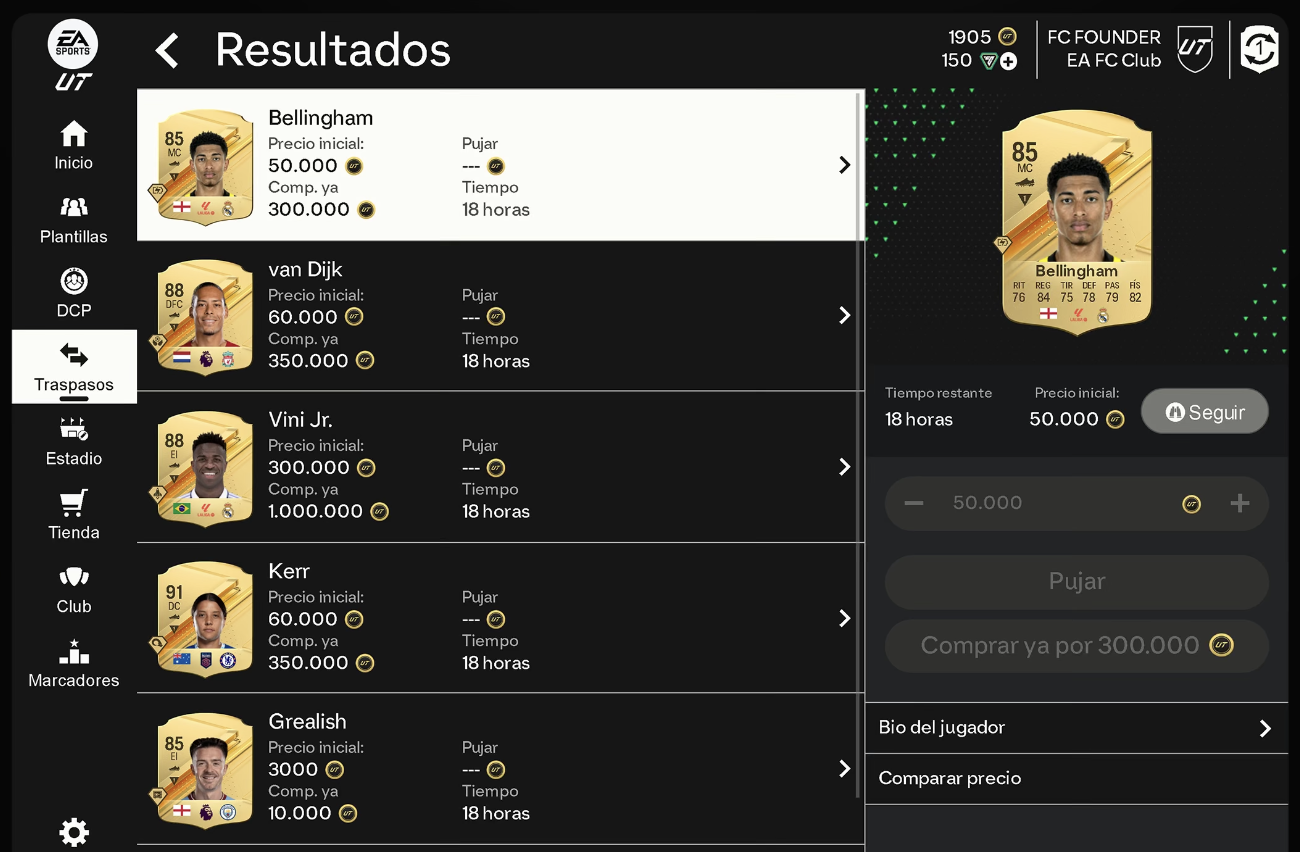
\includegraphics[width=0.7\textwidth]{figures/4-Estudio-viabilidad/4_FC_Companion.png}
    \caption{Página de traspasos de jugadores de EA SPORTS FC™ 24 Companion}
    \label{fig:ea_sports_fc_1}
    \hypertarget{fig:ea_sports_fc_1}{}
\end{figure}

\begin{figure}[H]
    \centering
    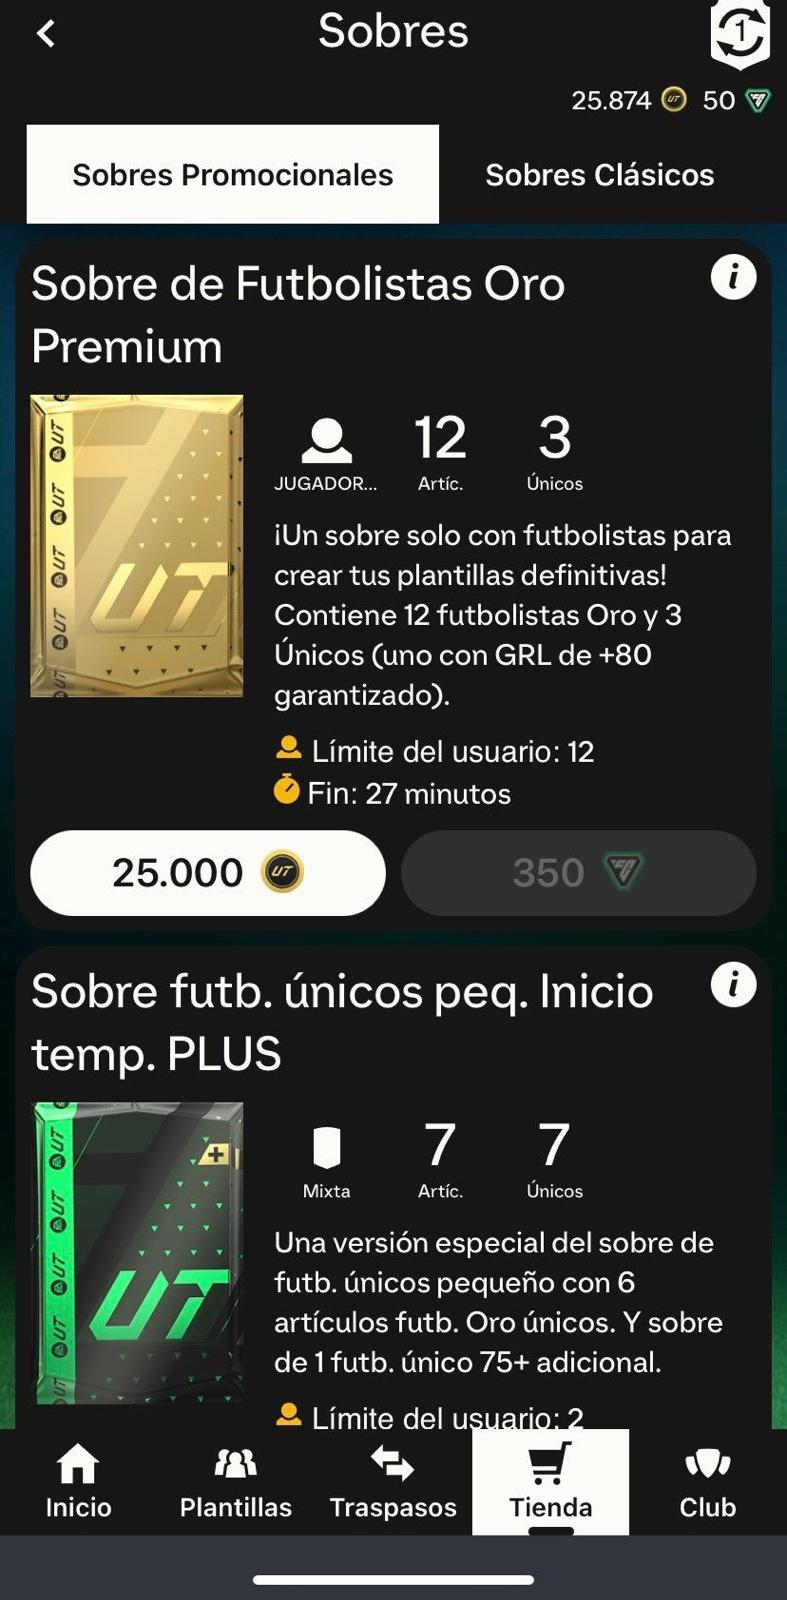
\includegraphics[width=0.3\textwidth]{figures/4-Estudio-viabilidad/4_FC_Companion2.jpeg}
    \caption{Página de compra de sobres de EA SPORTS FC™ 24 Companion}
    \label{fig:ea_sports_fc_2}
    \hypertarget{fig:ea_sports_fc_2}{}
\end{figure}

Por otra parte, EA SPORTS FC™ Mobile Fútbol es una versión adaptada de FIFA Ultimate Team para dispositivos móviles. Los usuarios pueden construir su equipo, competir en eventos y partidos en tiempo real, sin necesidad de haber comprado el juego físico.
Las compras están integradas en la aplicación, permitiendo a los usuarios adquirir monedas y puntos FIFA para mejorar su equipo, pero se pueden obtener de forma gratuita a través de eventos y desafíos.
Existe una tienda en la que los usuarios pueden comprar sobres de cartas por medio de dinero real o monedas del juego, así como un mercado de transferibles en el que pueden adquirir jugadores mediante subastas o compras directas.
También incorpora la opción de intercambiar cartas por cartas sorpresa.

En las siguientes capturas de pantalla, se muestra la interfaz de usuario de EA SPORTS FC™ Mobile Fútbol.
\begin{figure}[H]
    \centering
    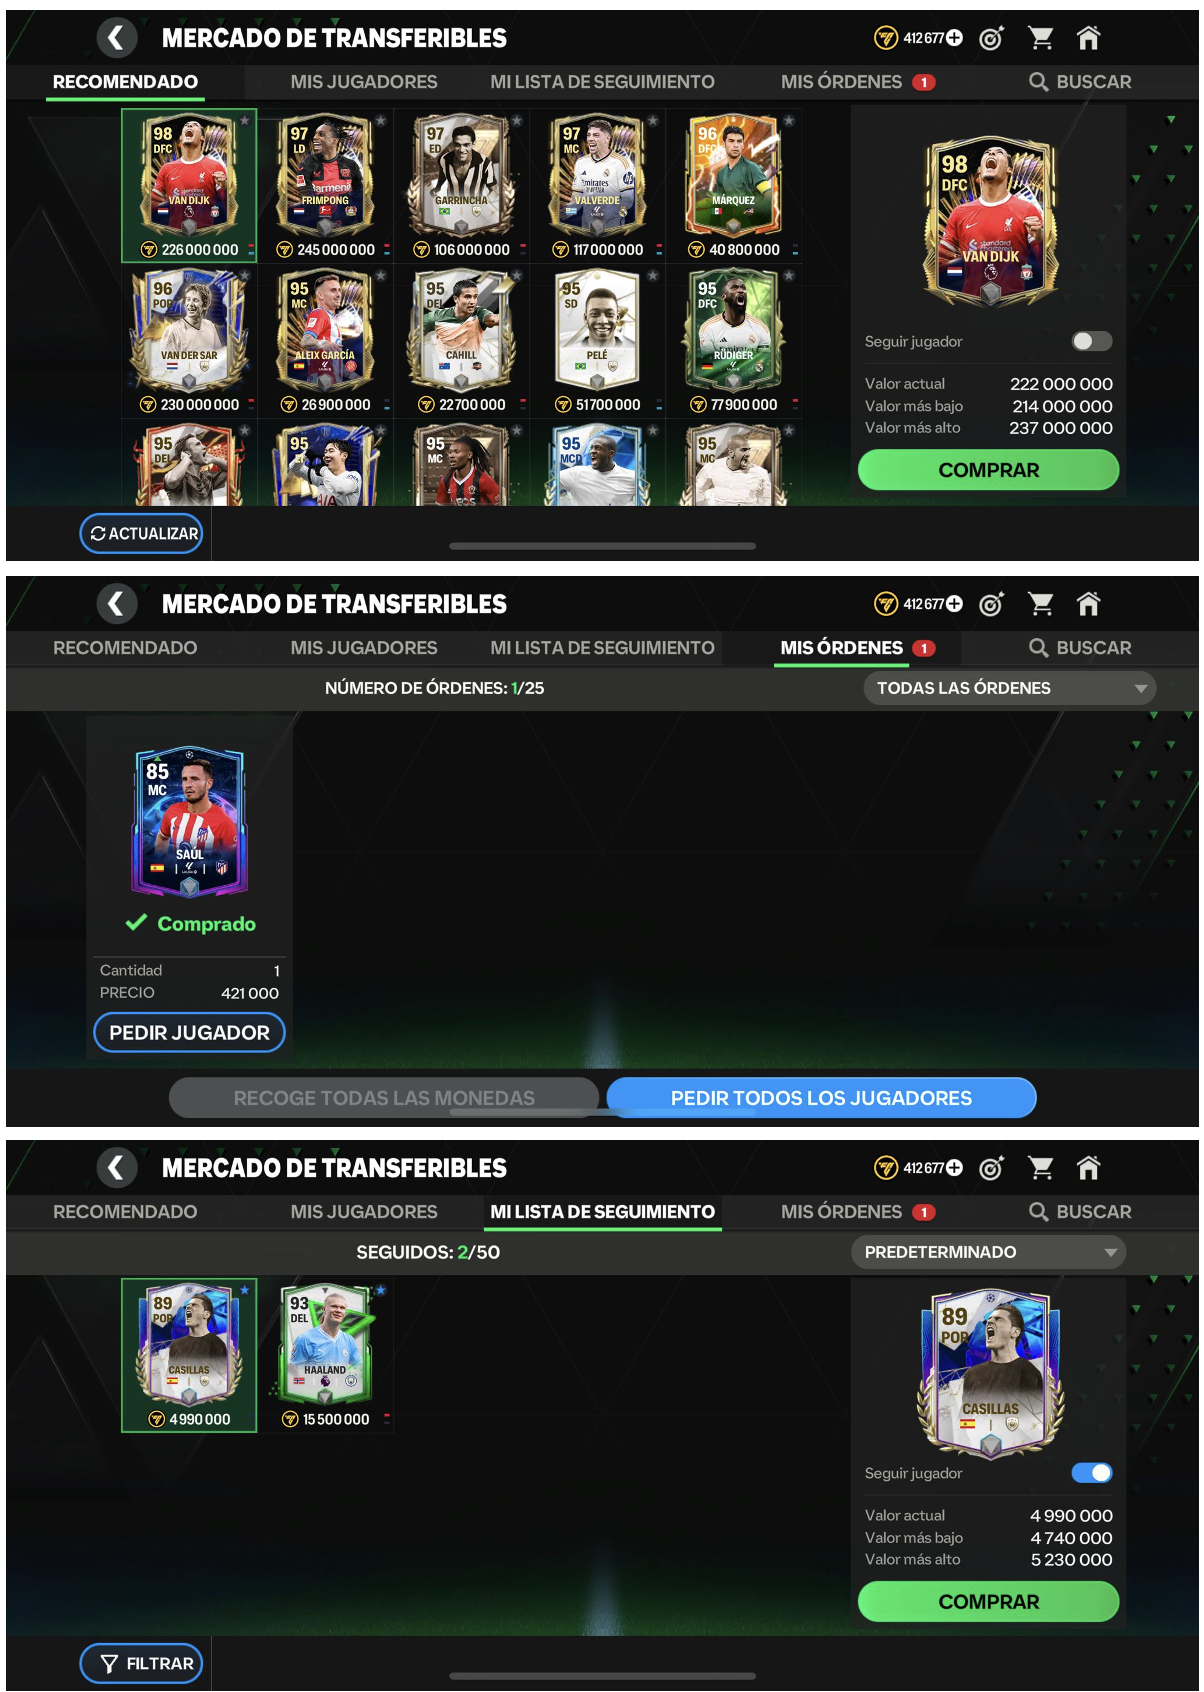
\includegraphics[width=0.7\textwidth]{figures/4-Estudio-viabilidad/4_FC_Mercado.png}
    \caption{Página de mercado de jugadores de EA SPORTS FC™ Mobile Fútbol}
    \label{fig:ea_sports_fc_mobile}
    \hypertarget{fig:ea_sports_fc_mobile}{}
\end{figure}

\begin{figure}[H]
    \centering
    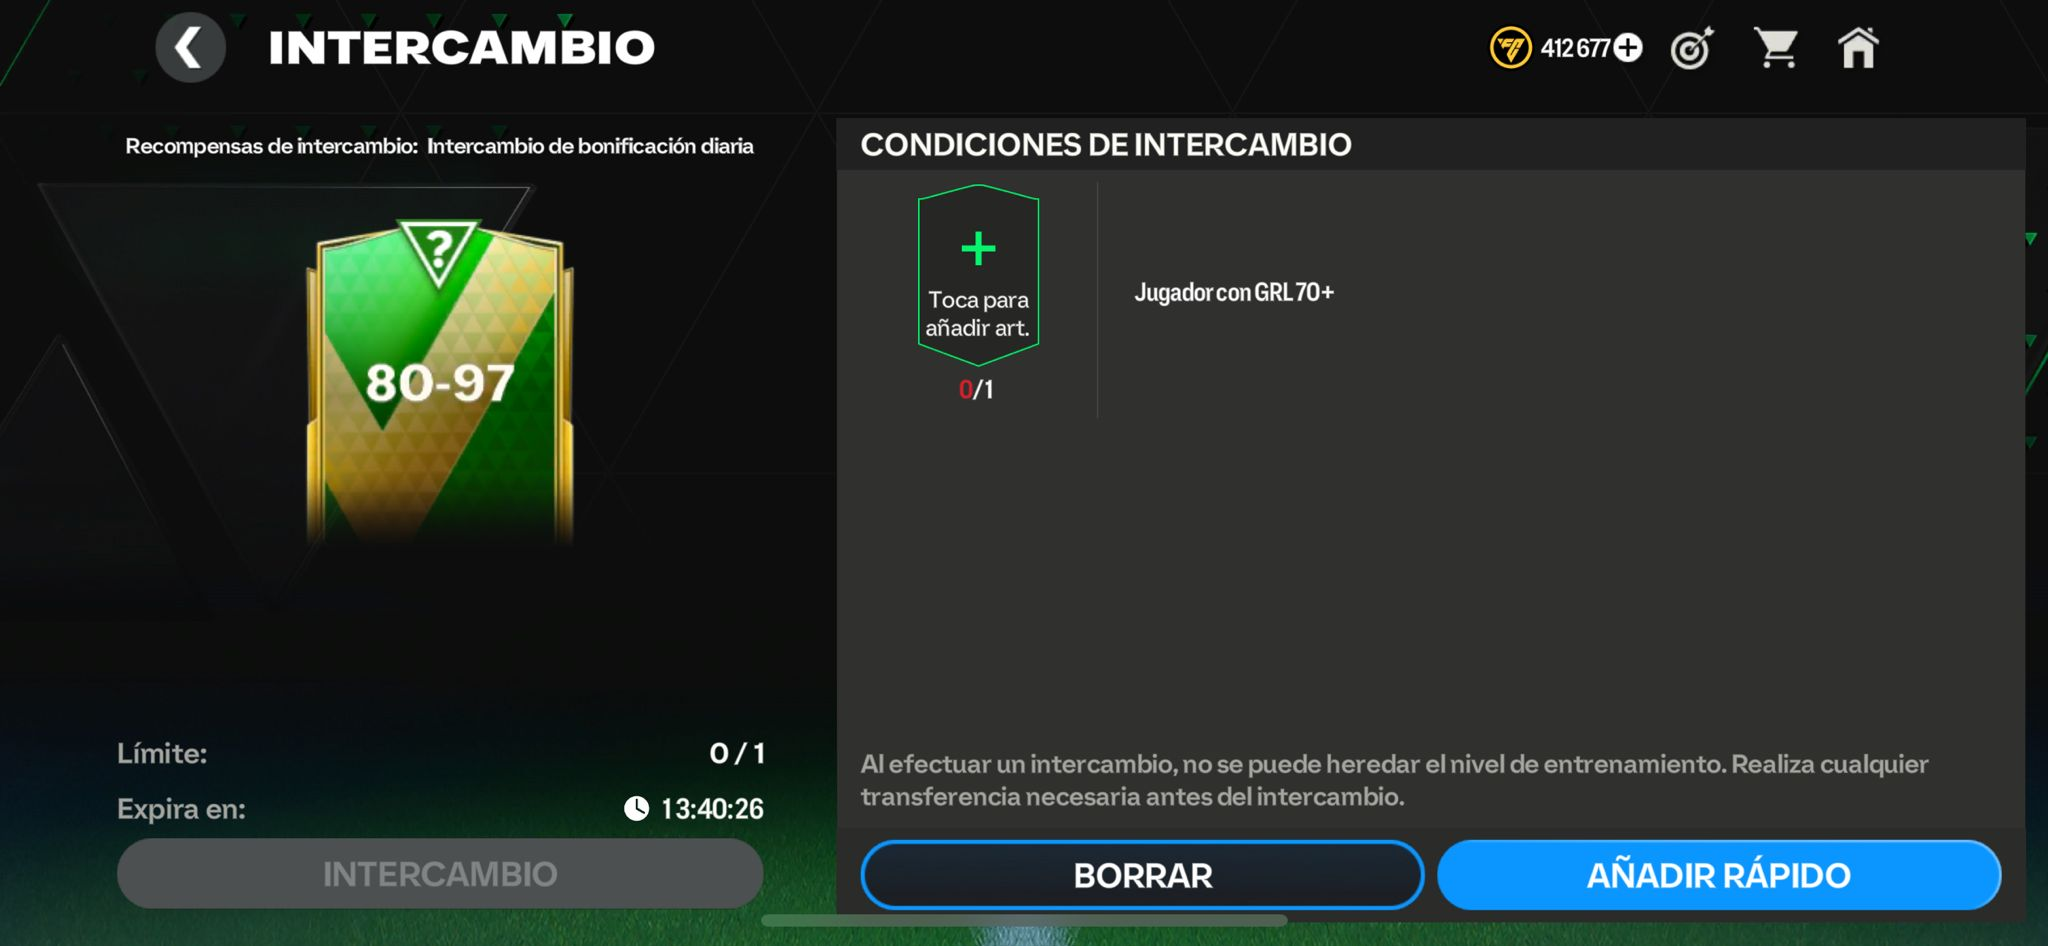
\includegraphics[width=0.7\textwidth]{figures/4-Estudio-viabilidad/4_FC-Intercambio.jpeg}
    \caption{Página de intercambio de cartas de EA SPORTS FC™ Mobile Fútbol}
    \label{fig:ea_sports_fc_mobile_2}
    \hypertarget{fig:ea_sports_fc_mobile_2}{}
\end{figure}

A continuación, se presentan las ventajas y desventajas de EA SPORTS FC™ Mobile Fútbol, así como las ventajas del nuevo sistema respecto a este. 
El motivo de centrarse en EA SPORTS FC™ Mobile Fútbol en lugar de la aplicación EA SPORTS FC™ 24 Companion es que la primera es una versión gratuita y accesible para todos los usuarios, además tienen características similares.

\subsubsubsection{Ventajas de EA SPORTS FC™ Mobile Fútbol}
En el contexto de EA SPORTS FC™ Mobile Fútbol, destacan las siguientes ventajas:
\begin{itemize}
    \item Los usuarios pueden marcar una carta para efectuar un seguimiento y recibir notificaciones en caso de una disminución en su precio.
    \item Se proporcionan estadísticas detalladas de cada carta, incluyendo su evolución de precio en las últimas semanas, así como los valores más bajos y más altos a los que se está vendiendo actualmente.
    \item Existe la opción de vender una carta directamente, evitando la necesidad de utilizar el sistema de subastas. 
    \item Cuenta con un buscador de ofertas que incorpora varios filtros.
    \item Los usuarios tienen la posibilidad de editar o cancelar sus pujas en curso.
    \item El sistema de subastas implementado opera bajo un mecanismo de puja ciega.
    \item La aplicación lanza ofertas de intercambio de cartas, permitiendo a los usuarios cambiar una o varias cartas que cumplan con ciertos requisitos por una carta sorpresa.
\end{itemize}

\subsubsubsection{Desventajas de EA SPORTS FC™ Mobile Fútbol}
Sin embargo, es importante mencionar algunas desventajas de EA SPORTS FC™ Mobile Fútbol, que incluyen:
\begin{itemize}
    \item Un número limitado de órdenes de canje simultáneas como, por ejemplo, el máximo de 25 permitido en EA Sports FC Mobile.
    \item Las pujas solo se pueden realizar por un valor igual o superior al establecido por el juego. 
    \item Existen varios tipos de monedas, lo que hace que no puedas conseguir ciertas cartas si no pagas por esas monedas ya que son muy díficiles de conseguir de forma gratuita.
\end{itemize}

\subsubsubsection{Ventajas del nuevo sistema respecto EA Sports FC}
El sistema en desarrollo presenta varias características que mejoran la experiencia del usuario en comparación con EA Sports FC.

\begin{itemize}
    \item El acceso a la aplicación es completamente gratuito.
    \item Ofrece una mayor personalización en el proceso de puja, brindando a los usuarios una experiencia más flexible y adaptada a sus preferencias.
    \item El usuario tiene la posibilidad de acceder a un histórico exhaustivo en el que se detallan todas las transacciones realizadas.
\end{itemize}

\subsubsection{NBA 2K}
\coloredUnderline{\href{https://nba.2k.com/}{NBA 2K}} es una destacada franquicia de videojuegos de baloncesto disponible en diversas plataformas. 
En esta sección se analizarán las aplicaciones \coloredUnderline{\href{https://nba.2k.com/2k24/mynba-2k24/}{MyNBA 2K Companion App}} y \coloredUnderline{\href{https://nba.2k.com/2k24/es-ES/myteam/}{NBA 2K24 MyTEAM}}.

MyTEAM busca transformar la interacción de los jugadores, permitiéndoles construir y gestionar su propio equipo de baloncesto. Los usuarios pueden buscar jugadores en la tienda de la aplicación, para mejorar su equipo y competir en eventos y partidos en tiempo real.
Existen distintos niveles de cartas para añadir un elemento de emoción al juego y cartas de recompensa que se pueden obtener completando desafíos y eventos especiales.

Se estima que NBA 2K ha generado ingresos significativos en los últimos años. En el año fiscal 2023, 
los ingresos de Take-Two Interactive alcanzaron niveles récord gracias a sus franquicias principales, incluyendo NBA 2K. El informe anual de Take-Two Interactive para el año fiscal 2023\cite{take_two_2023} 
destaca que NBA 2K es una de las mayores fuentes de ingresos de la empresa, con una base de usuarios activa y comprometida, especialmente en el modo MyTEAM. 
En el informe se menciona la intención de seguir desarrollando este mercado ya que se espera que continúe creciendo en los próximos años.

La popularidad de este modo de juego ha llevado a Take-Two Interactive a lanzar una aplicación móvil llamada MyNBA 2K Companion App. Es una aplicación gratuita, pero los usuarios necesitan tener el juego NBA 2K para utilizarla.
La aplicación permite canjear códigos a los usuarios para obtener recompensas en el juego, así como consultar estadísticas de su saldo sin necesidad de iniciar sesión en la consola.
Tiene otras funciones interesantes como la posibilidad de personalizar su propio jugador por medio de la función de escaneo facial, la cual permite a los usuarios escanear su rostro y añadirlo al juego.


En la siguiente figura, se muestra la interfaz de usuario de MyNBA 2K Companion App.
\begin{figure}[H]
    \centering
    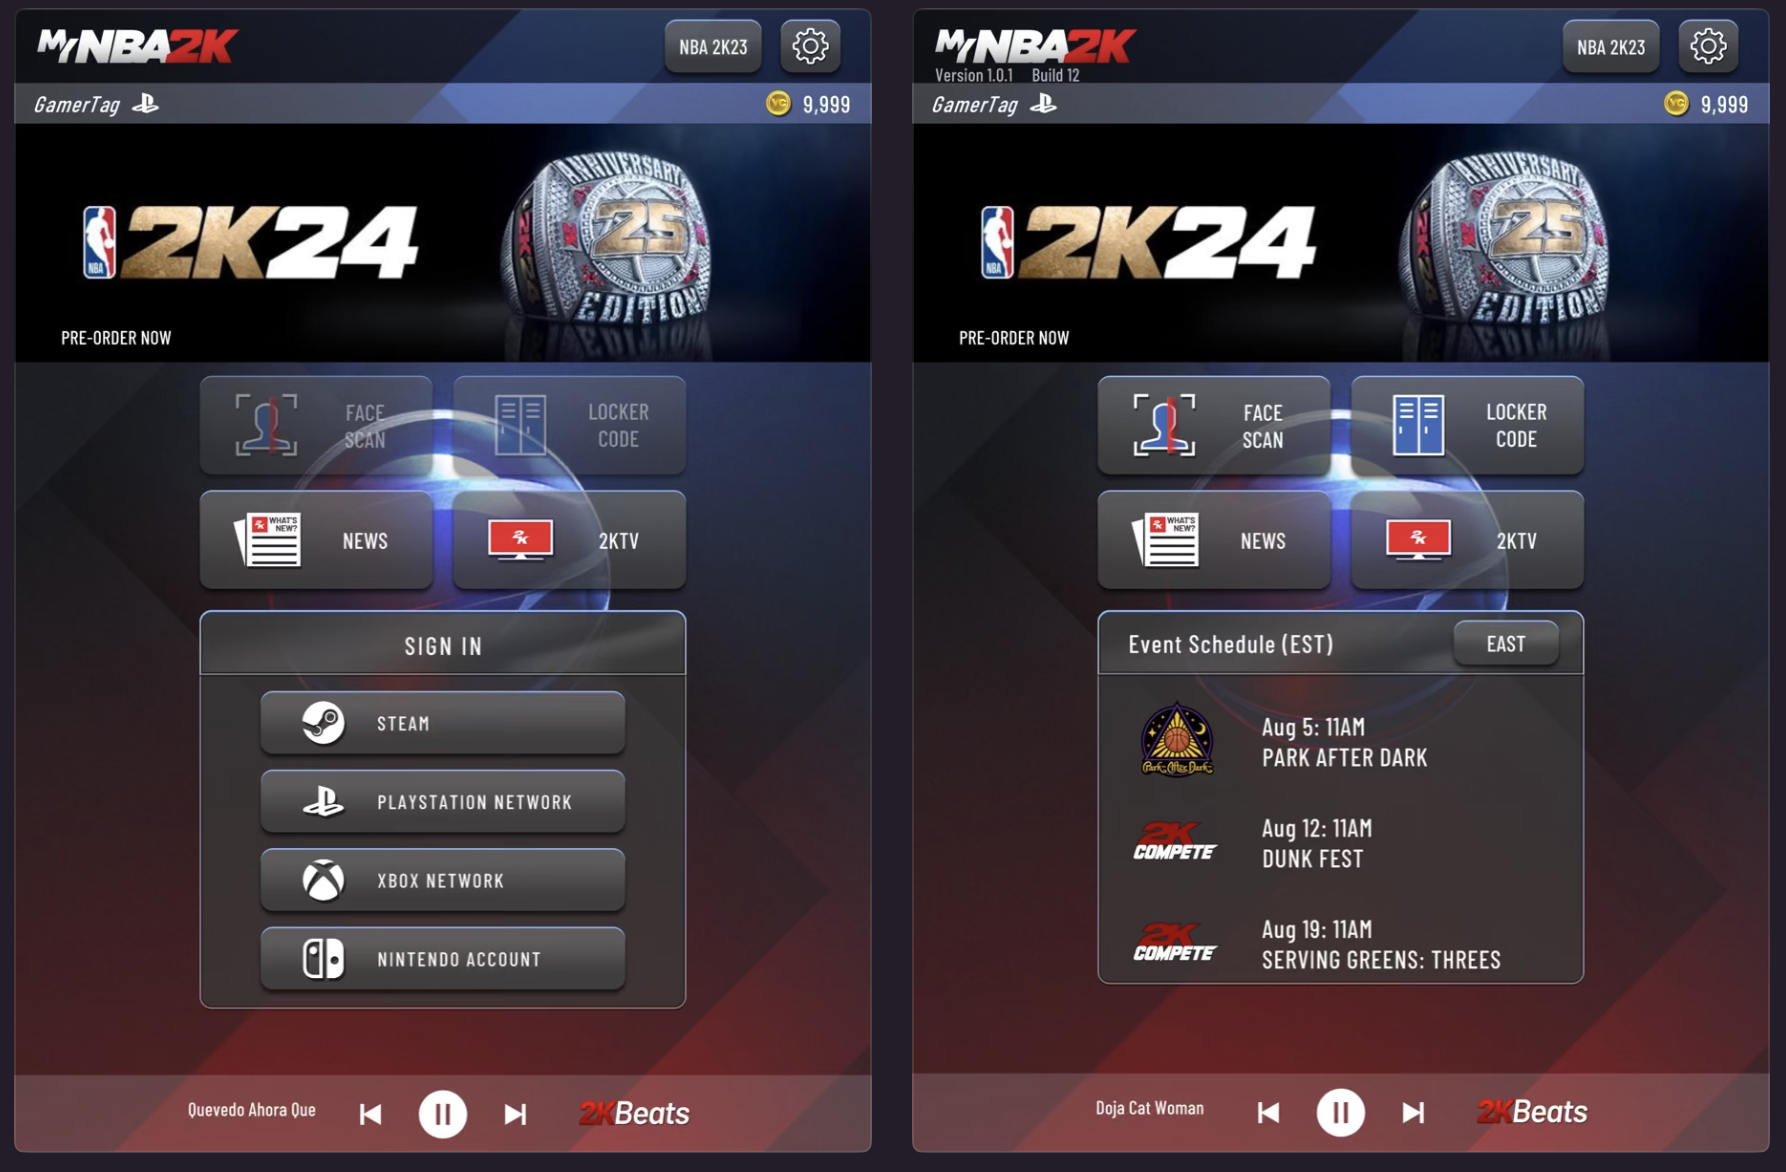
\includegraphics[width=0.7\textwidth]{figures/4-Estudio-viabilidad/4_NBA.png}
    \caption{Página de mercado de jugadores de MyNBA 2K Companion App}
    \label{fig:nba_2k}
    \hypertarget{fig:nba_2k}{}
\end{figure}

Por otra parte, NBA 2K24 MyTEAM es una versión adaptada de MyTEAM que perimite registarse y jugar sin necesidad de tener el juego NBA 2K. 
Los usuarios pueden construir su equipo, competir en eventos y partidos, y mejorar su equipo mediante la adquisición de jugadores en la tienda de la aplicación. 
No pueden realizar subastas ni vender cartas, pero se permite el intercambio de cartas repetidas por cartas sorpresa.

En las siguientes capturas de pantalla, se muestra la interfaz de usuario de NBA 2K24 MyTEAM.
\begin{figure}[H]
    \centering
    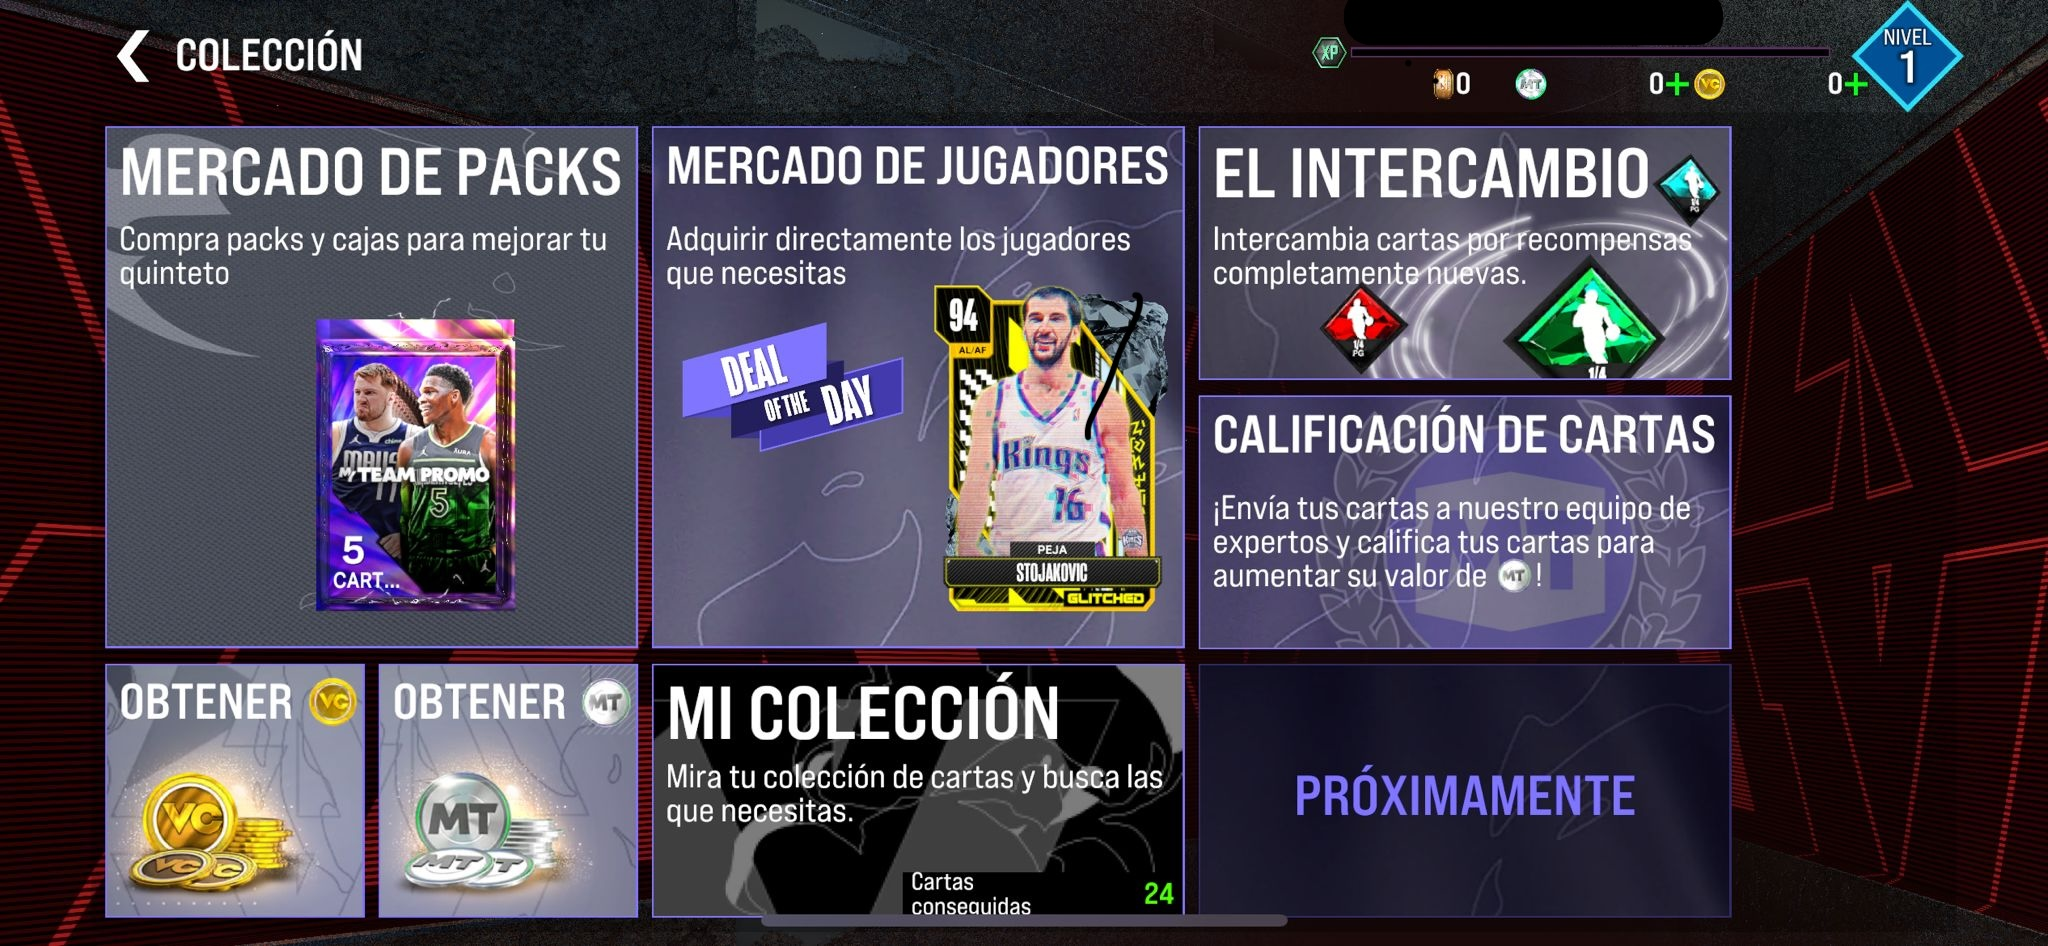
\includegraphics[width=0.7\textwidth]{figures/4-Estudio-viabilidad/4_NBA2.jpeg}
    \caption{Página de colección de jugadores de NBA 2K24 MyTEAM}
    \label{fig:nba_2k_2}
    \hypertarget{fig:nba_2k_2}{}
\end{figure}

A continuación, se presentan las ventajas y desventajas de NBA 2K24 MyTEAM, así como las ventajas del nuevo sistema respecto a este. 
Se ha decidido centrarse en NBA 2K24 MyTEAM en lugar de MyNBA 2K Companion App, ya que la primera es una versión gratuita y accesible para todos los usuarios.

\subsubsubsection{Ventajas de NBA 2K24 MyTEAM}
En el contexto de NBA 2K, destacan las siguientes ventajas:
\begin{itemize}
    \item Se pueden buscar jugadores en la tienda de la aplicación y adquirirlos para mejorar el equipo.
    \item Existe la opción de intercambiar cartas repetidas por cartas sorpresa.
\end{itemize}

\subsubsubsection{Desventajas de NBA 2K24 MyTEAM}
Sin embargo, es importante mencionar algunas desventajas de NBA 2K, que incluyen:
\begin{itemize}
    \item No hay un mercado de subastas en el que los usuarios puedan adquirir jugadores mediante pujas ni vender cartas.
    \item Existen dos tipos de monedas en el juego, una de pago y otra gratuita, lo que puede hacer que no puedas comprar cierta carta o acceder a ciertas características del juego si no pagas.
\end{itemize}

\subsubsubsection{Ventajas del nuevo sistema respecto NBA 2K}
El sistema en desarrollo presenta varias características que mejoran la experiencia del usuario en comparación con NBA 2K.
\begin{itemize}
    \item Ofrece la opción de subasta de cartas, brindando a los usuarios una experiencia más flexible y adaptada a sus preferencias.
    \item Solo se utilizará una moneda en el juego, lo que facilita la adquisición de cartas y sobres.
\end{itemize}

\subsubsection{LaLiga Fantasy}
\coloredUnderline{\href{https://laligafantasy.relevo.com/}{LaLiga Fantasy}} un juego basado en la liga de fútbol española, conocida como LaLiga. En este juego, los usuarios tienen la capacidad de crear equipos que se componen de jugadores cuyo rendimiento se correlaciona con el desempeño real en los partidos de LaLiga. Además, existe la posibilidad de competir por premios reales en determinadas instancias del juego.
El juego dispone de un mercado en el que los usuarios pueden vender o adquirir jugadores a través de un sistema de subastas, por lo que estamos ante un escenario similar al anterior.

A continuación, se muestra la interfaz de usuario de LaLiga Fantasy.
\begin{figure}[H]
    \centering
    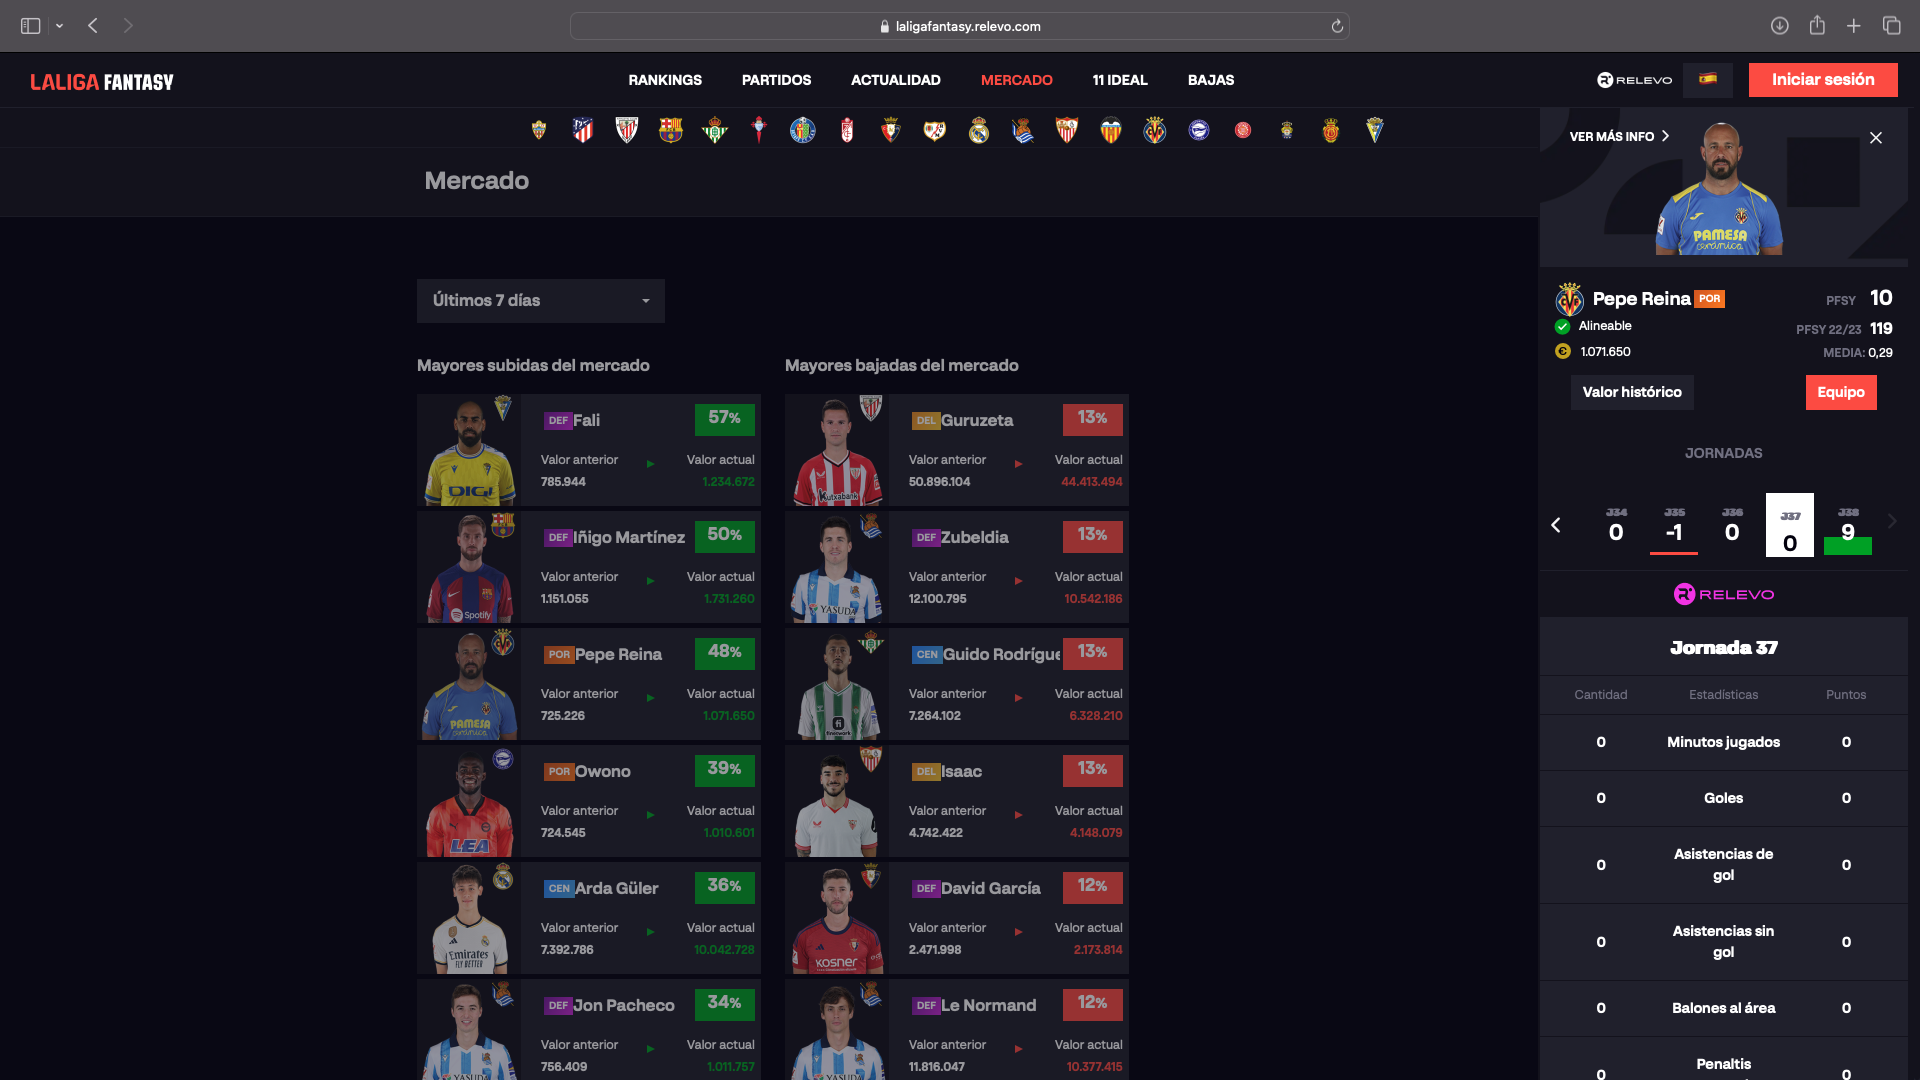
\includegraphics[width=0.7\textwidth]{figures/4-Estudio-viabilidad/4_LaLigaFantasy.png}
    \caption{Página de mercado de jugadores de LaLiga Fantasy}
    \label{fig:la_liga_fantasy}
    \hypertarget{fig:la_liga_fantasy}{}
\end{figure}

\subsubsubsection{Ventajas de LaLiga Fantasy}
Dentro del marco de LaLiga Fantasy, se destacan las siguientes características:
\begin{itemize}
    \item El juego renueva constantemente el mercado de transferibles.
    \item El juego cuenta con la capacidad de generar ofertas automáticas por los futbolistas que se encuentran en venta. Estas ofertas se establecen a partir de un valor aleatorio que oscila entre el valor de mercado del jugador, con un margen del 10\% tanto por encima como por debajo de dicho valor.
    \item Recientemente se ha incorporado el mercado de ``clausulazos'', donde los usuarios pueden adquirir un jugador pagando su cláusula, que será más elevada que el valor de mercado, sin tener que depender del propietario del jugador.
    \item Se pueden realizar ofertas por jugadores a otros usuarios.
\end{itemize}

\subsubsubsection{Desventajas de LaLiga Fantasy}
Se pueden identificar las siguientes desventajas:
\begin{itemize}
    \item La limitación a un máximo de 24 jugadores en la plantilla, lo que puede ocasionar la pérdida de oportunidades en subastas.
    \item La plataforma brinda escasa flexibilidad en lo que respecta a la personalización al momento de poner un jugador en venta.
\end{itemize}

\subsubsubsection{Ventajas del nuevo sistema respecto LaLiga Fantasy}
\begin{itemize}
    \item LaLiga Fantasy ofrece una suscripción de 0,99€/mes para poder jugar sin anuncios mientras que el sistema que se desarrollará carece de anuncios.
    \item Se proporciona un historial de transacciones completo para que los usuarios puedan rastrear las compras y ventas.
    \item Se implementa un sistema de subastas en tiempo real que, además, brinda una mayor personalización al usuario en aspectos como la duración de la subasta y los valores de venta, entre otros.
    \item Además de acceder al mercado, los usuarios tienen la opción de adquirir sobres de cartas, lo que añade un elemento de emoción a la aplicación.
\end{itemize}



\subsection{Análisis de sistemas de subastas en línea}
\subsubsection{eBay}
\coloredUnderline{\href{https://www.ebay.es/}{eBay}} es una plataforma de comercio online que permite a los usuarios comprar y vender productos a través de subastas o ventas directas. 
Es una de las plataformas de venta \textit{online} más grandes y conocidas del mundo, con una amplia variedad de productos disponibles, desde artículos de colección hasta productos de consumo diario.

En el primer trimestre de 2024, eBay ha reportado varias métricas financieras clave \cite{ebay2024} que reflejan su desempeño sólido y su amplia adopción global. 
La plataforma cuenta con 132 millones de compradores activos a nivel mundial, lo que subraya su extensa base de usuarios y el interés que genera en el mercado.
Los ingresos totales para el primer trimestre de 2024 fueron de 2.6 billones de dólares, demostrando la robustez del modelo de negocio de eBay. 
Desde esta plataforma los vendedores tienen la opción de establecer un precio fijo por su producto o permitir que los compradores pujen por él.

La plataforma ofrece dos opciones para comprar un producto. La primera es la compra directa, en la que el comprador adquiere el producto al precio establecido por el vendedor, y la segunda es la subasta, en la que los compradores pujan por el producto y el comprador con la puja más alta al final del tiempo de la subasta se lleva el producto.

En el caso de las subastas, eBay permite a los vendedores establecer el precio base, que es el precio mínimo al que están dispuestos a vender el producto y también tienen la opción de establecer un precio de compra directa, que es el precio al que un comprador puede adquirir el producto sin necesidad de pujar.

La aplicación permite a los compradores hacer seguimiento de los productos que les interesan, recibir notificaciones sobre el estado de las subastas y pujar por productos de forma automática, estableciendo un precio máximo.

Ofrece información en tiempo real sobre las subastas, como el número de pujas, el precio actual, el tiempo restante y el número de pujadores. Además, proporciona un historial de las pujas realizadas en un producto, lo que permite a los compradores ver cómo ha evolucionado el precio y quiénes han pujado.
También permite a los usuarios consultar las valoraciones de los vendedores y ver los productos que tienen en venta.

En la siguiente figura, se muestra la interfaz de usuario de la sección de coleccionismo de cartas de eBay.
\begin{figure}[H]
    \centering
    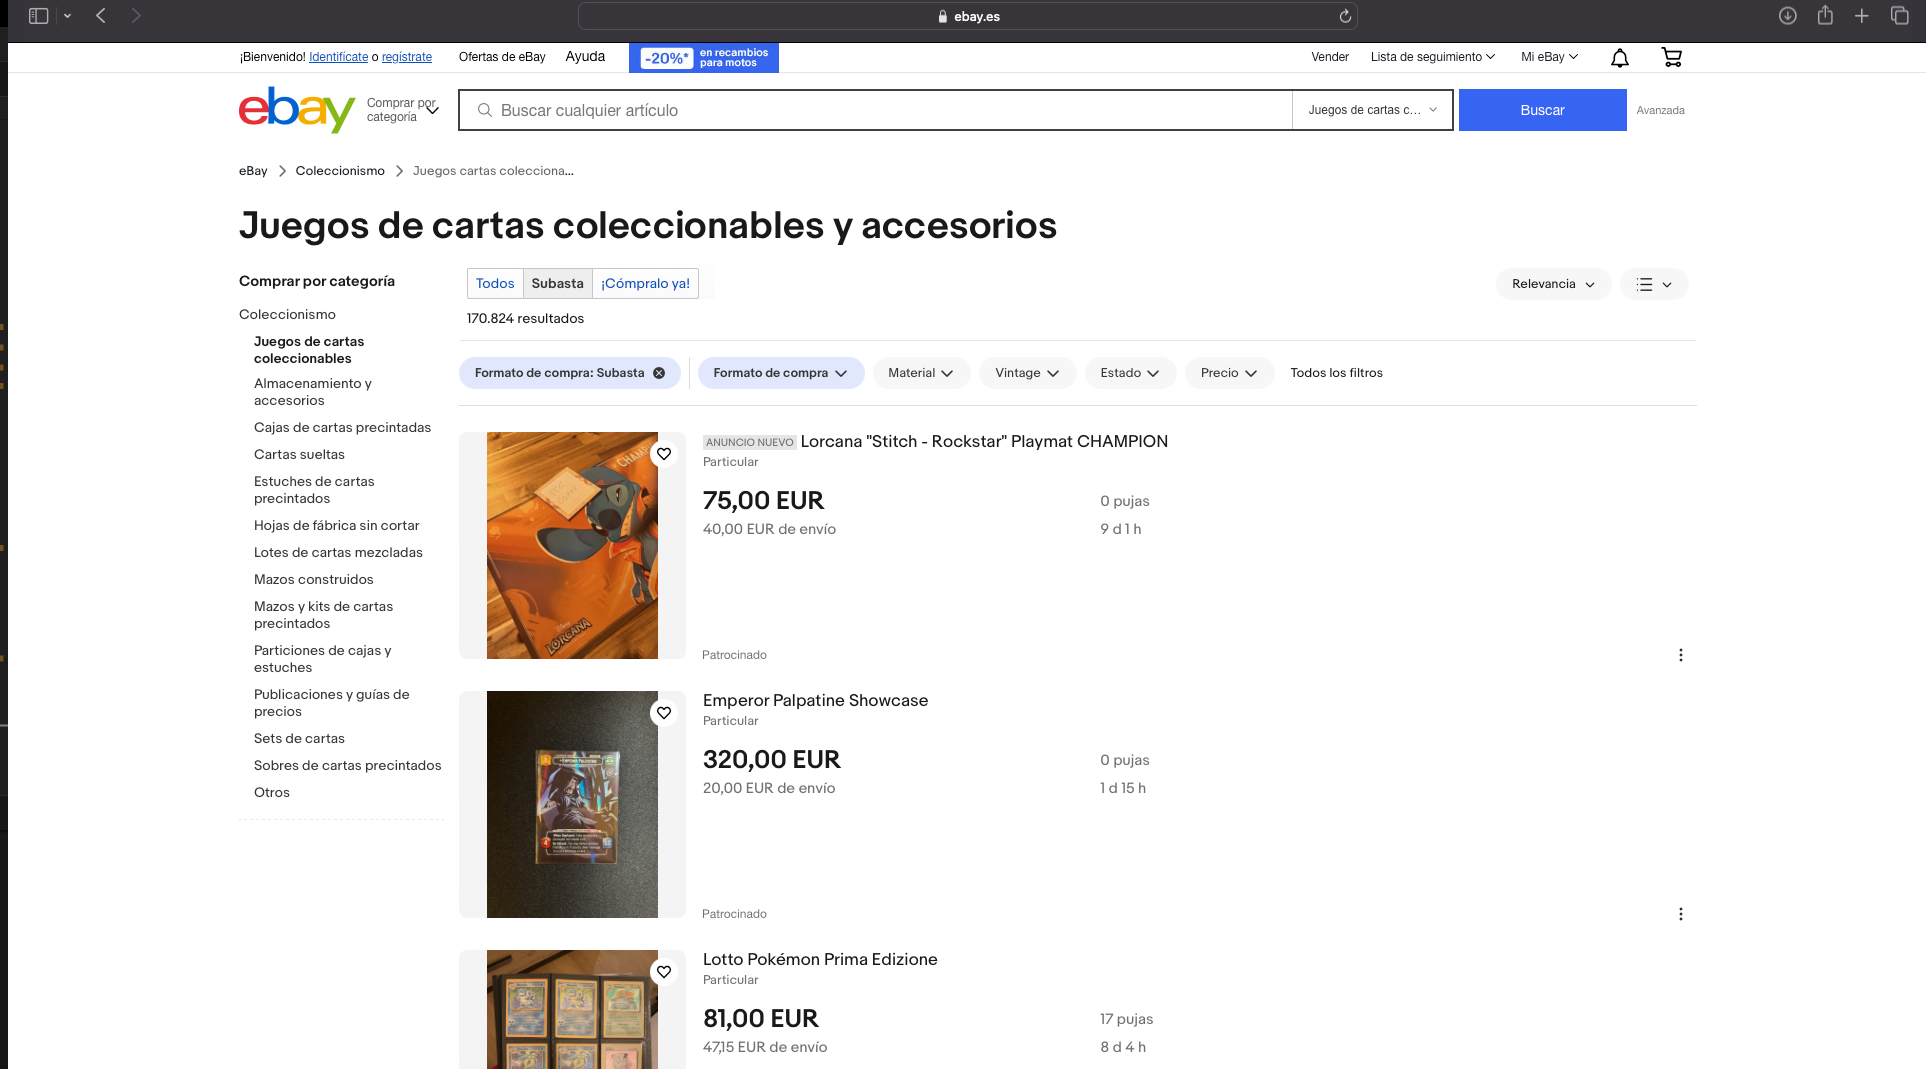
\includegraphics[width=0.9\textwidth]{figures/4-Estudio-viabilidad/4_Ebay.png}
    \caption{Página de subastas de la sección de coleccionismo de cartas de eBay}
    \label{fig:ebay}
    \hypertarget{fig:ebay}{}
\end{figure} 

\subsubsubsection{Ventajas de eBay}
Dentro del marco de LaLiga Fantasy, se destacan las siguientes características:
\begin{itemize}
    \item Para cada producto subastado, la plataforma ofrece la posibilidad de visualizar información detallada que incluye el número de pujas, la cantidad de pujadores, las retractaciones, el tiempo restante en la subasta, y proporciona un historial completo de las pujas realizadas en ese producto. Este historial incluye datos relevantes sobre las pujas, como su valor y la fecha en la que se efectuaron. Además, se brinda acceso a información pertinente sobre los pujadores involucrados.
    \item eBay proporciona a los usuarios la capacidad de configurar pujas automáticas. En este proceso, el comprador define el precio máximo que está dispuesto a pagar por el producto, y la plataforma aumenta automáticamente la oferta en su nombre, siempre que sea necesario, para mantener al comprador como el principal postor hasta alcanzar el límite previamente establecido.
    \item Los usuarios tienen la posibilidad de examinar el perfil del vendedor, explorar otros productos que este tenga en venta y establecer contacto directo con él.
    \item Como vendedor, la plataforma te brinda la capacidad de definir el valor inicial de la puja, decidir si deseas recibir ofertas, establecer la fecha de inicio de la subasta, determinar su duración y habilitar la opción de compra directa a un precio específico de tu elección.
\end{itemize}

\subsubsubsection{Desventajas de eBay}
A continuación, es posible señalar las siguientes desventajas:
\begin{itemize}
    \item La interfaz de usuario muestra una gran cantidad de información, lo que puede resultar confuso para alguien que no está acostumbrado a ella.
    \item Cuando se va a realizar una puja, no aparece una ventana emergente de confirmación de puja o similar por lo que es fácil introducir una puja errónea y, posteriormente, puede resultar complicado retirarla.
    \item Las subastas tienen incrementos de puja predefinidos, lo que significa que no puedes especificar un valor concreto por el que desees pujar.
\end{itemize}

\subsubsubsection{Ventajas del nuevo sistema respecto eBay}
\begin{itemize}
    \item El sistema en desarrollo presentará una interfaz simple e intuitiva, que proporcionará todos los datos esenciales para efectuar una puja con confianza, sin abrumar al usuario con una sobrecarga de información.
    \item El sistema que se desarrollará proporcionará al usuario información sobre las condiciones para retirar una puja antes de su confirmación.
\end{itemize}


\subsubsection{Catawiki}
\coloredUnderline{\href{https://www.catawiki.com/es/}{Catawiki}} es una plataforma de subastas online que permite a los usuarios comprar y vender productos de colección. 
La plataforma cuenta con varias secciones dedicadas a diferentes categorías de coleccionismo, tales como arte, relojes y cómics. 
Existe una sección específica dedicada al coleccionismo de cartas, donde los usuarios pueden pujar por cartas de interés, como las cartas de Pokémon.

La plataforma presenta una interfaz intuitiva y sencilla que permite a los usuarios pujar por cartas de manera rápida y eficaz. Según la propia empresa, 
posee más de 10 millones de compradores en todo el mundo, cuenta con aproximadamente 240 expertos encargados de la preparación de los objetos subastados, 
opera en 60 países y ofrece atención al cliente en 17 idiomas \cite{catawiki}. En base a esto, se puede afirmar que Catawiki es una plataforma consolidada y de confianza en el mercado de subastas \textit{online}.

El uso de la página web es gratuito, aunque se cobra una comisión por la venta de los productos subastados.
Los usuarios pueden establecer un precio mínimo de puja, denominado 'Precio de Reserva', que permanece oculto para los demás usuarios, 
permitiendo a los vendedores asegurarse de que no se venderá por debajo de un precio determinado. 
Si se realiza una puja en un lote con un precio de reserva, la plataforma informará al usuario que no se ha alcanzado dicho precio y ofrecerá la opción de aumentar su puja.

Los vendedores pueden consultar de forma transparente las comisiones que se aplicarán en caso de que se venda el producto. 
En general, la página web recibe buenas opiniones por parte de los usuarios, quienes destacan la seguridad que ofrece al realizar transacciones.

La aplicación cuenta con aproximadamente 240 expertos en las diferentes categorías de objetos subastados. 
Estos expertos revisan virtualmente los objetos enviados, ayudan a los vendedores con la presentación de los objetos y responden a las preguntas de los compradores.

Al acceder a un objeto subastado, se puede consultar quién lo vende y qué experto lo ha supervisado, además se pueden ver las pujas realizadas y el tiempo restante para que finalice la subasta. 
En algunos casos, en la información relativa al objeto aparece el valor que el experto considera que tiene el objeto, lo que puede ayudar a los compradores a decidir si pujar por el objeto.

Es posible ver comentarios acerca del vendedor y la reputación que tiene en la plataforma, lo que puede influir en la decisión de los compradores al pujar por un objeto.

La plataforma también ofrece la opción de pujar de forma automática, estableciendo un precio máximo, y se encargará de pujar por el usuario hasta alcanzar dicho precio. 
La interfaz informa sobre la reputación del vendedor, el número de pujas realizadas y la fecha de finalización de la subasta.

Las pujas son vinculantes, la plataforma informa de que si se gana una subasta, el usuario está obligado a comprar el objeto. Esto puede ser un aspecto a tener en cuenta, ya que si se gana una subasta,
se deberá abonar el importe correspondiente al objeto subastado.

En resumen, ofrece bastante información sobre los objetos subastados y los vendedores, lo que puede ayudar a los compradores a tomar una decisión informada. Además, posee una interfaz sencilla y fácil de usar, lo que facilita la navegación por la plataforma.


En la \coloredUnderline{\hyperlink{fig:catawiki}{Figura \ref*{fig:catawiki}:\nameref*{fig:catawiki}}} se muestra la interfaz de usuario de la sección de coleccionismo de cartas de Pokémon Catawiki.

\begin{figure}[H]
    \centering
    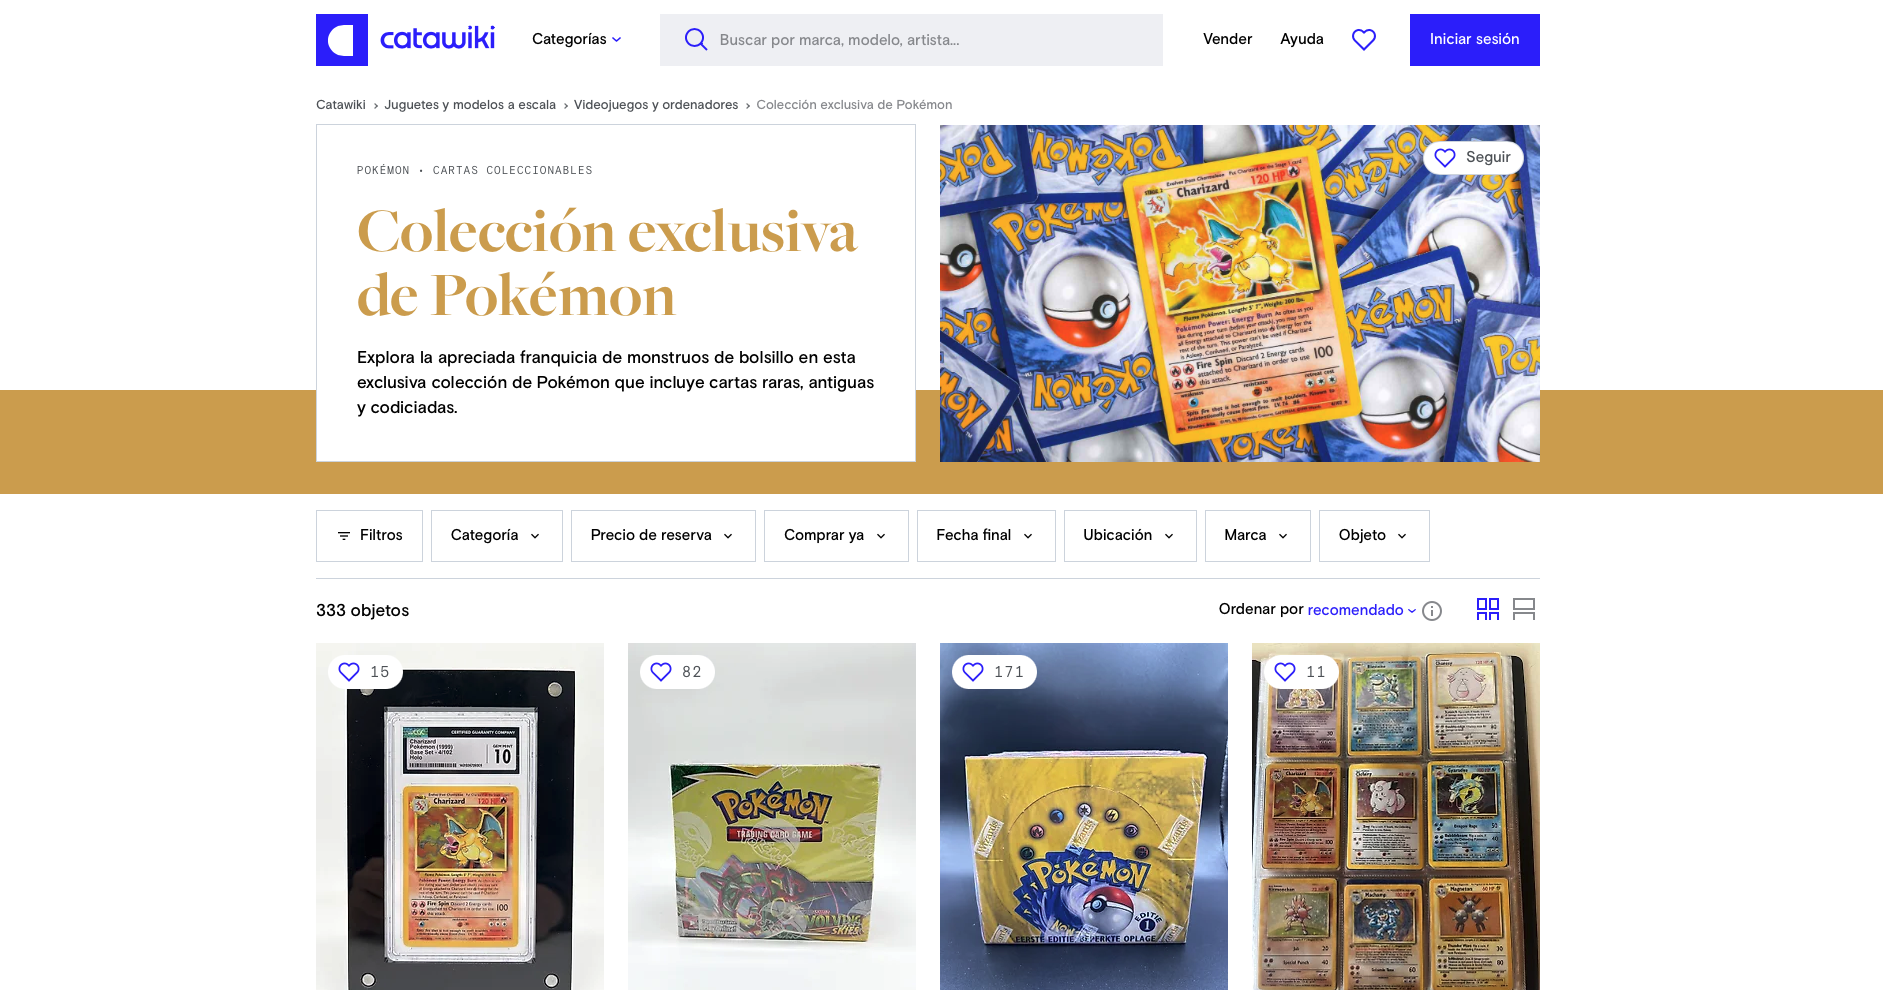
\includegraphics[width=0.9\textwidth]{figures/4-Estudio-viabilidad/4_Catawiki.png}
    \caption{Página de subastas de la sección de coleccionismo de cartas Pokémon de Catawiki}
    \label{fig:catawiki}
    \hypertarget{fig:catawiki}{}
\end{figure}

En la \coloredUnderline{\hyperlink{fig:catawiki2}{Figura \ref*{fig:catawiki2}:\nameref*{fig:catawiki2}}} se muestra la interfaz de usuario de la subasta de una carta de Pokémon en Catawiki.
\begin{figure}[H]
    \centering
    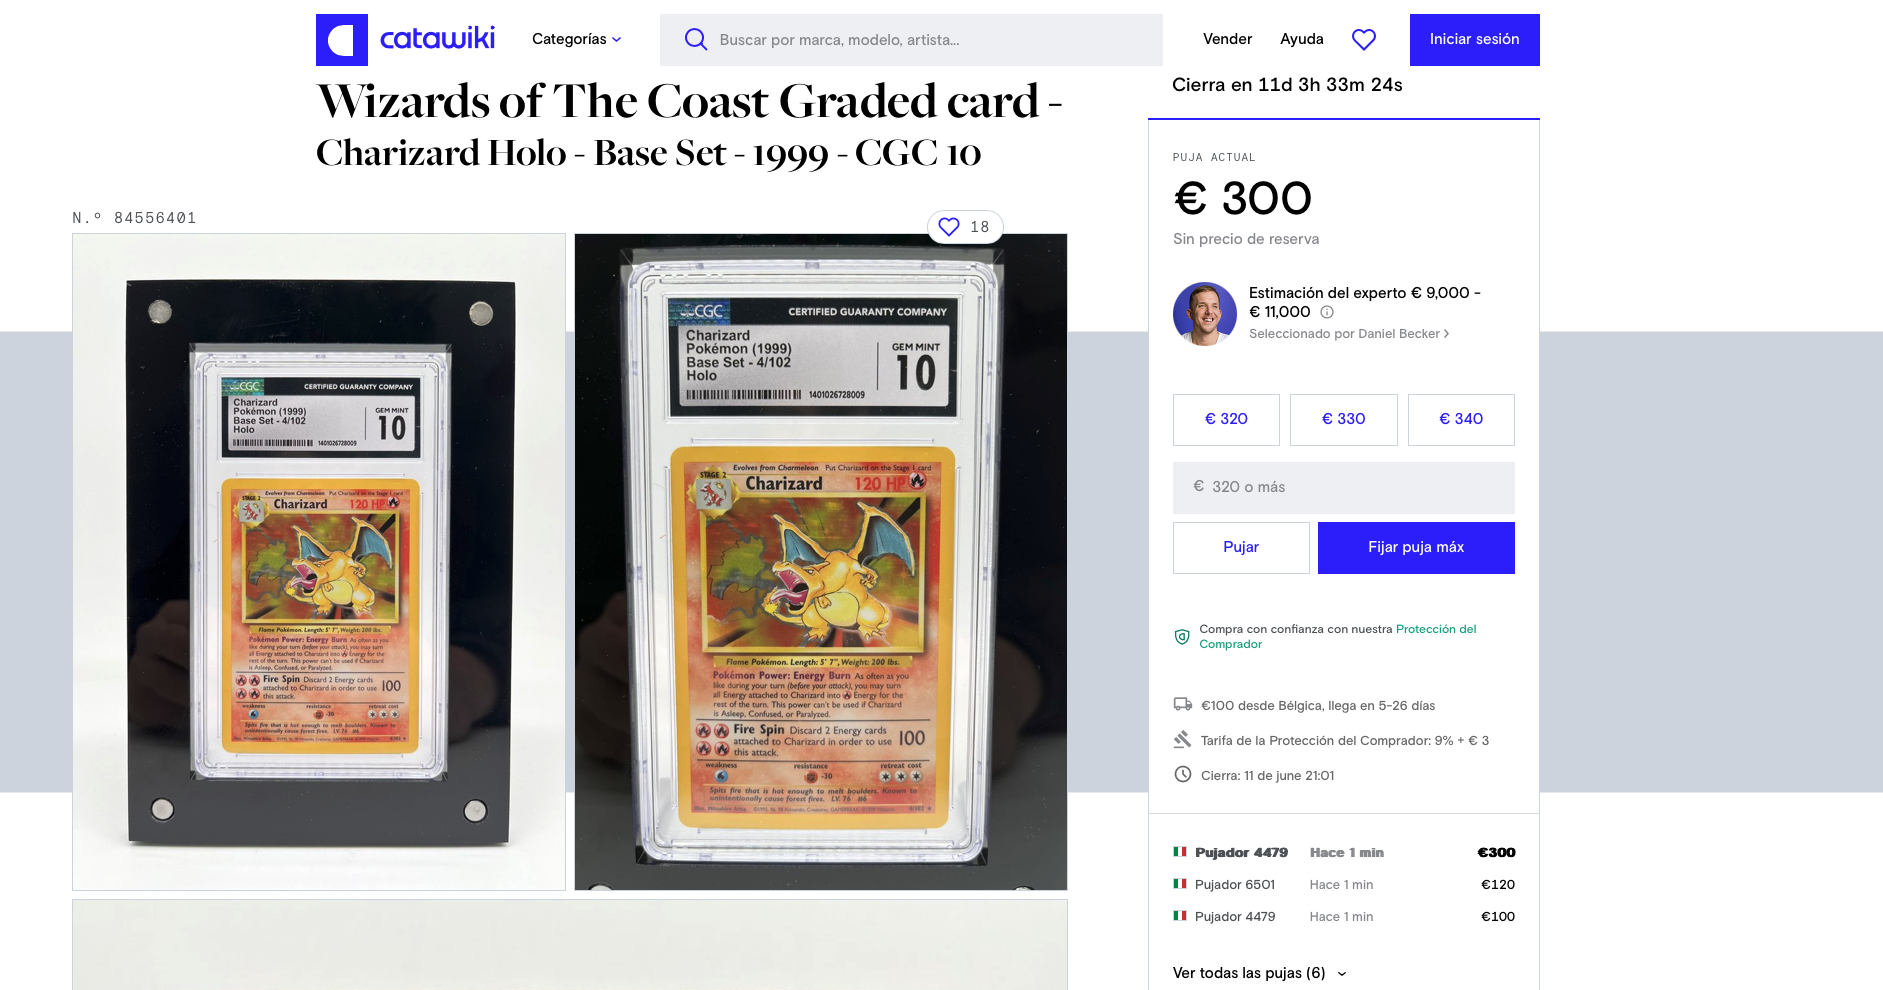
\includegraphics[width=0.9\textwidth]{figures/4-Estudio-viabilidad/4_Catawiki-puja.png}
    \caption{Página de subasta de una carta de Pokémon en Catawiki}
    \label{fig:catawiki2}
    \hypertarget{fig:catawiki2}{}
\end{figure}

\subsubsubsection{Ventajas de Catawiki}
Dentro del marco de Catawiki, se destacan las siguientes características:
\begin{itemize}
    \item La plataforma ofrece una amplia variedad de objetos de colección, lo que permite a los usuarios encontrar productos de su interés.
    \item Los usuarios pueden consultar la reputación del vendedor y la valoración junto con comentarios que ha recibido de otros compradores.
    \item La plataforma ofrece la posibilidad de pujar de forma automática, estableciendo un precio máximo, lo que facilita la participación en las subastas.
    \item Los expertos de la plataforma revisan los objetos subastados, lo que puede ayudar a los compradores a tomar una decisión informada y sentirse seguros al realizar una puja.
\end{itemize}

\subsubsubsection{Desventajas de Catawiki}
A continuación, es posible señalar las siguientes desventajas:
\begin{itemize}
    \item Las pujas son vinculantes, lo que significa que si se gana una subasta, el usuario está obligado a comprar el objeto.
    Una vez realizada una puja no se puede retirar ni modificar, lo que puede ser un problema si se ha pujado por error o si se ha cambiado de opinión.
    \item Algunos clientes se quejan de que los precios de envío, comisiones y otros gastos adicionales pueden ser elevados, lo que puede aumentar en exceso el precio final del objeto.
\end{itemize}

\subsubsubsection{Ventajas del nuevo sistema respecto Catawiki}
Algunos de los elementos que diferencian al sistema en desarrollo de Catawiki benefician a los usuarios y mejoran su experiencia en la plataforma son los siguientes:
\begin{itemize}
    \item El sistema en desarrollo permitirá a los usuarios retirar una puja antes de que finalice la subasta, lo que puede ser útil si se ha pujado por error o si se ha cambiado de opinión.
    \item La plataforma que se desarrollará no cobrará comisiones por la venta de los productos subastados, lo que puede resultar atractivo para los usuarios. 
\end{itemize}


% https://www.pwccmarketplace.com/weekly-auction?category=pokemonenglish-pokemonjapanese-pokemonotherlanguage plataforma de subastas de cartas de pokemon certificadas

\subsection{El mercado de coleccionistas de Pokémon}

El mercado de coleccionistas de Pokémon es un sector en constante crecimiento y expansión. La popularidad de las cartas de Pokémon ha aumentado significativamente en los últimos años, 
lo que ha llevado a un incremento en la demanda de cartas de colección y a un aumento en los precios de las cartas más raras y valiosas. Las plataformas de subastas en línea han contribuido 
notablemente a esta expansión, permitiendo a los coleccionistas comprar y vender cartas de Pokémon de forma segura y eficiente. 

Estas plataformas, a menudo, emplean intermediarios encargados de verificar la autenticidad de las cartas y de garantizar la seguridad de las transacciones, 
brindando a los coleccionistas mayor confianza al realizar compras y ventas.

Existen varias plataformas web que ofrecen análisis detallados de los precios de las cartas de Pokémon, como \coloredUnderline{\href{https://www.pokemonprice.com/MarketCap}{PokemonPrice}} y \coloredUnderline{\href{https://www.pricecharting.com/console/pokemon-base-set}{PriceCharting}}. 
Estas plataformas permiten a los coleccionistas consultar el valor de mercado de las cartas de Pokémon, así como el precio de venta de las cartas más populares y raras. 
Además, proporcionan historiales de precios y gráficos que muestran la evolución del precio de las cartas a lo largo del tiempo. 
Los datos se actualizan regularmente, recopilando información de plataformas de ventas como eBay.

En la \coloredUnderline{\hyperlink{fig:pokemonprice}{Figura \ref*{fig:pokemonprice}:\nameref*{fig:pokemonprice}}} se muestra el análisis de precios de las cartas de Pokémon de PokemonPrice.

\begin{figure}[H]
    \centering
    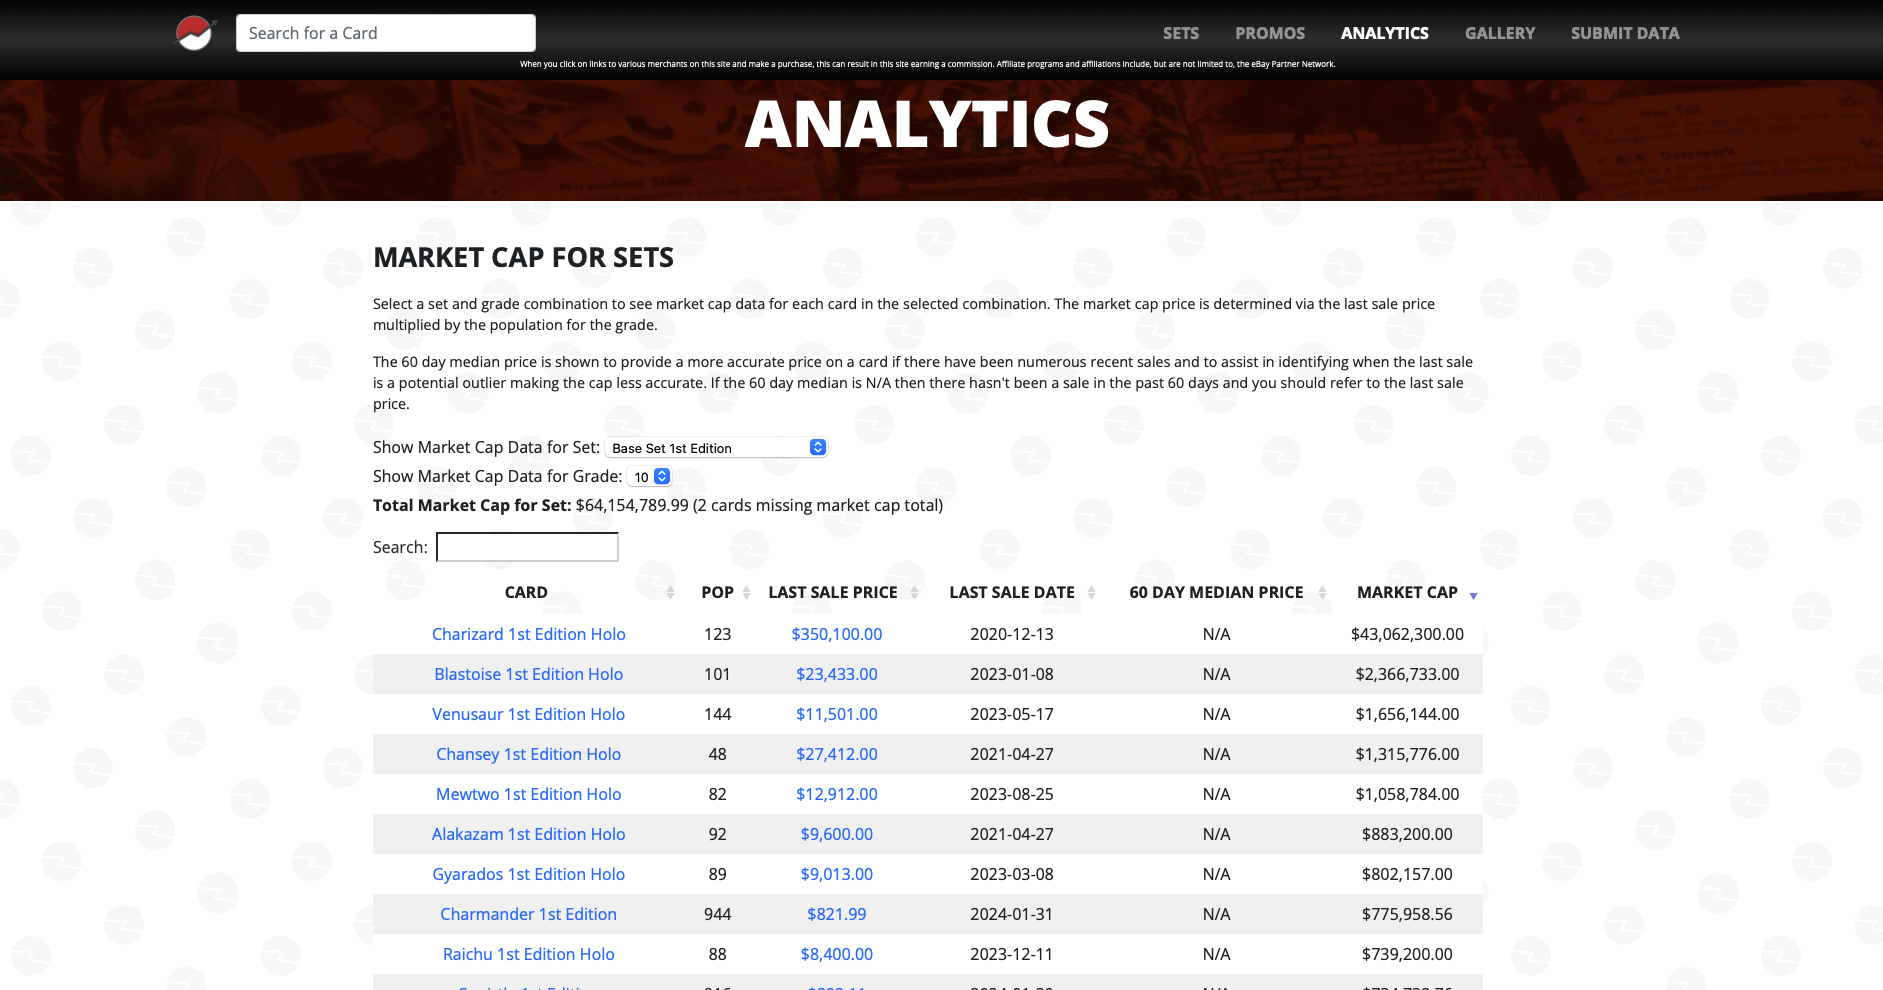
\includegraphics[width=0.9\textwidth]{figures/4-Estudio-viabilidad/4_PokemonPrice.png}
    \caption{Página de cartas de Pokémon de PokemonPrice}
    \label{fig:pokemonprice}
    \hypertarget{fig:pokemonprice}{}
\end{figure}

En esta plataforma, los usuarios pueden ver el precio de mercado de una carta concreta y las transacciones realizadas, como se muestra en la \coloredUnderline{\hyperlink{fig:pokemonprice2}{Figura \ref*{fig:pokemonprice2}:\nameref*{fig:pokemonprice2}}}.

\begin{figure}[H]
    \centering
    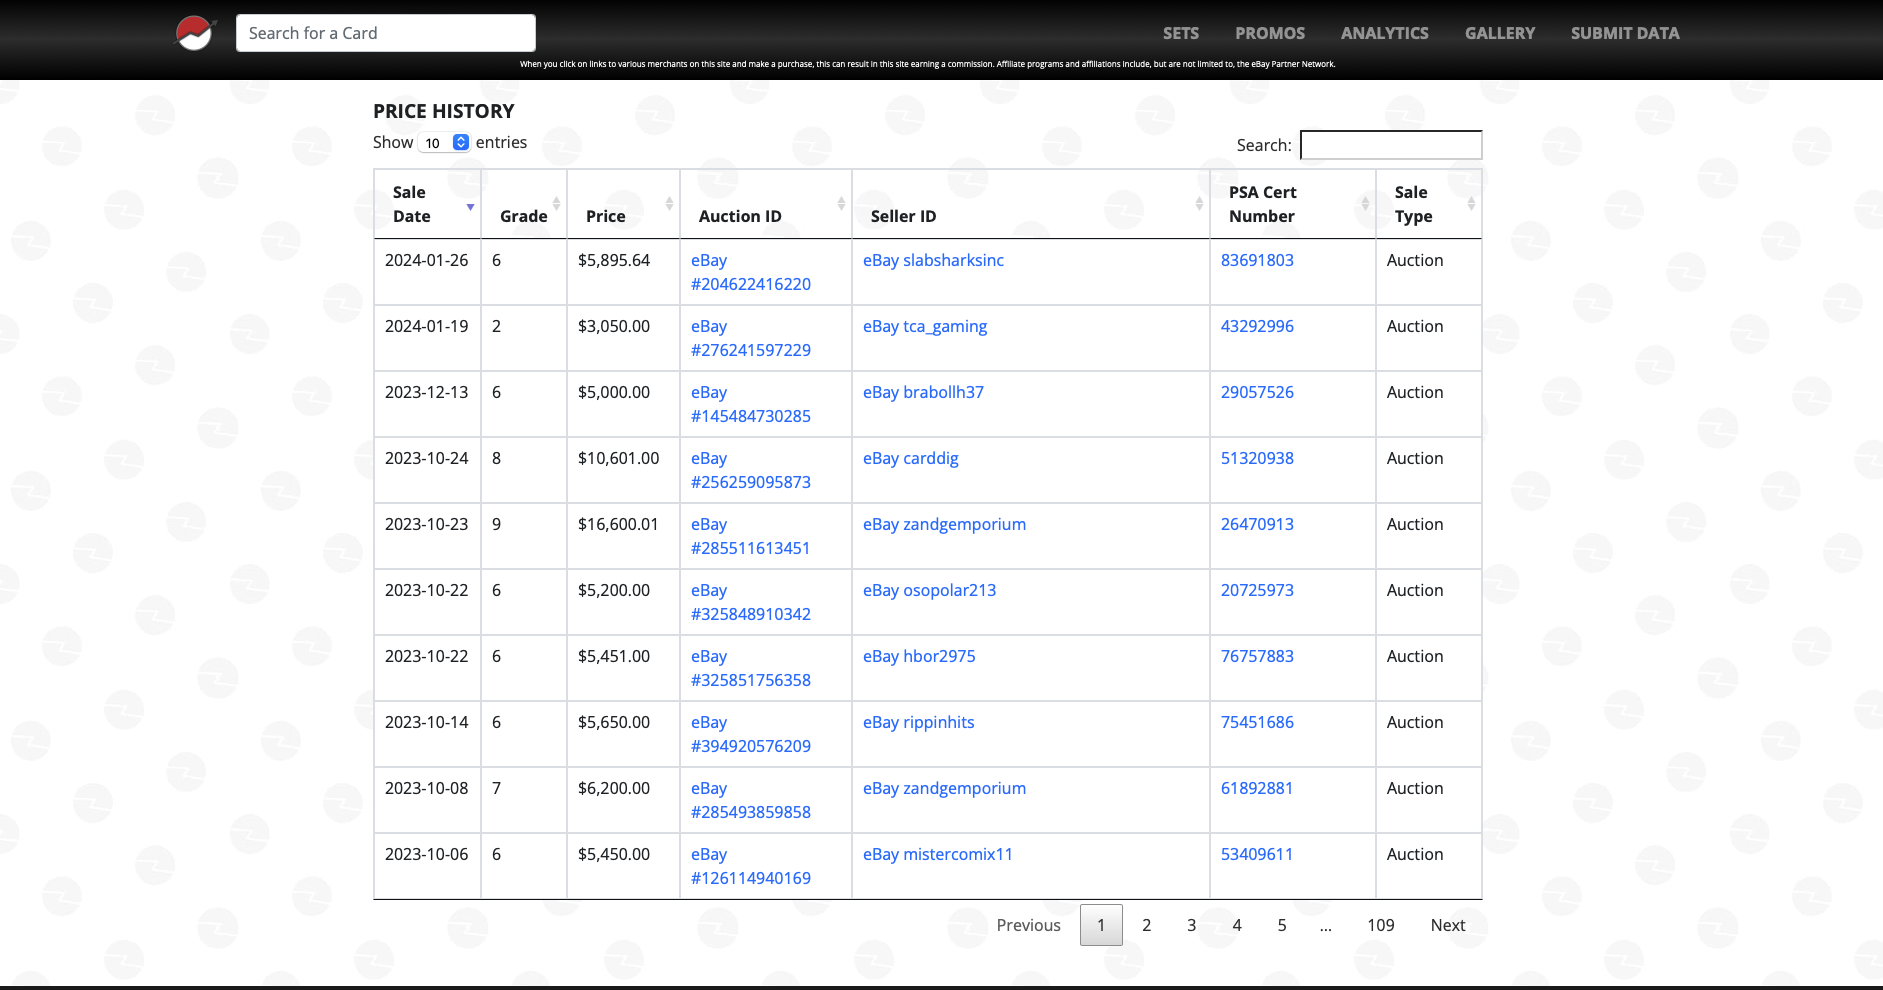
\includegraphics[width=0.9\textwidth]{figures/4-Estudio-viabilidad/4_PokemonPrice2.png}
    \caption{Página de una carta de Pokémon de PokemonPrice}
    \label{fig:pokemonprice2}
    \hypertarget{fig:pokemonprice2}{}
\end{figure}

En la \coloredUnderline{\hyperlink{fig:pricecharting}{Figura \ref*{fig:pricecharting}:\nameref*{fig:pricecharting}}} se muestra la interfaz de usuario de consulta de datos para un set
 de cartas de Pokémon de la plataforma PriceCharting.

\begin{figure}[H]
    \centering
    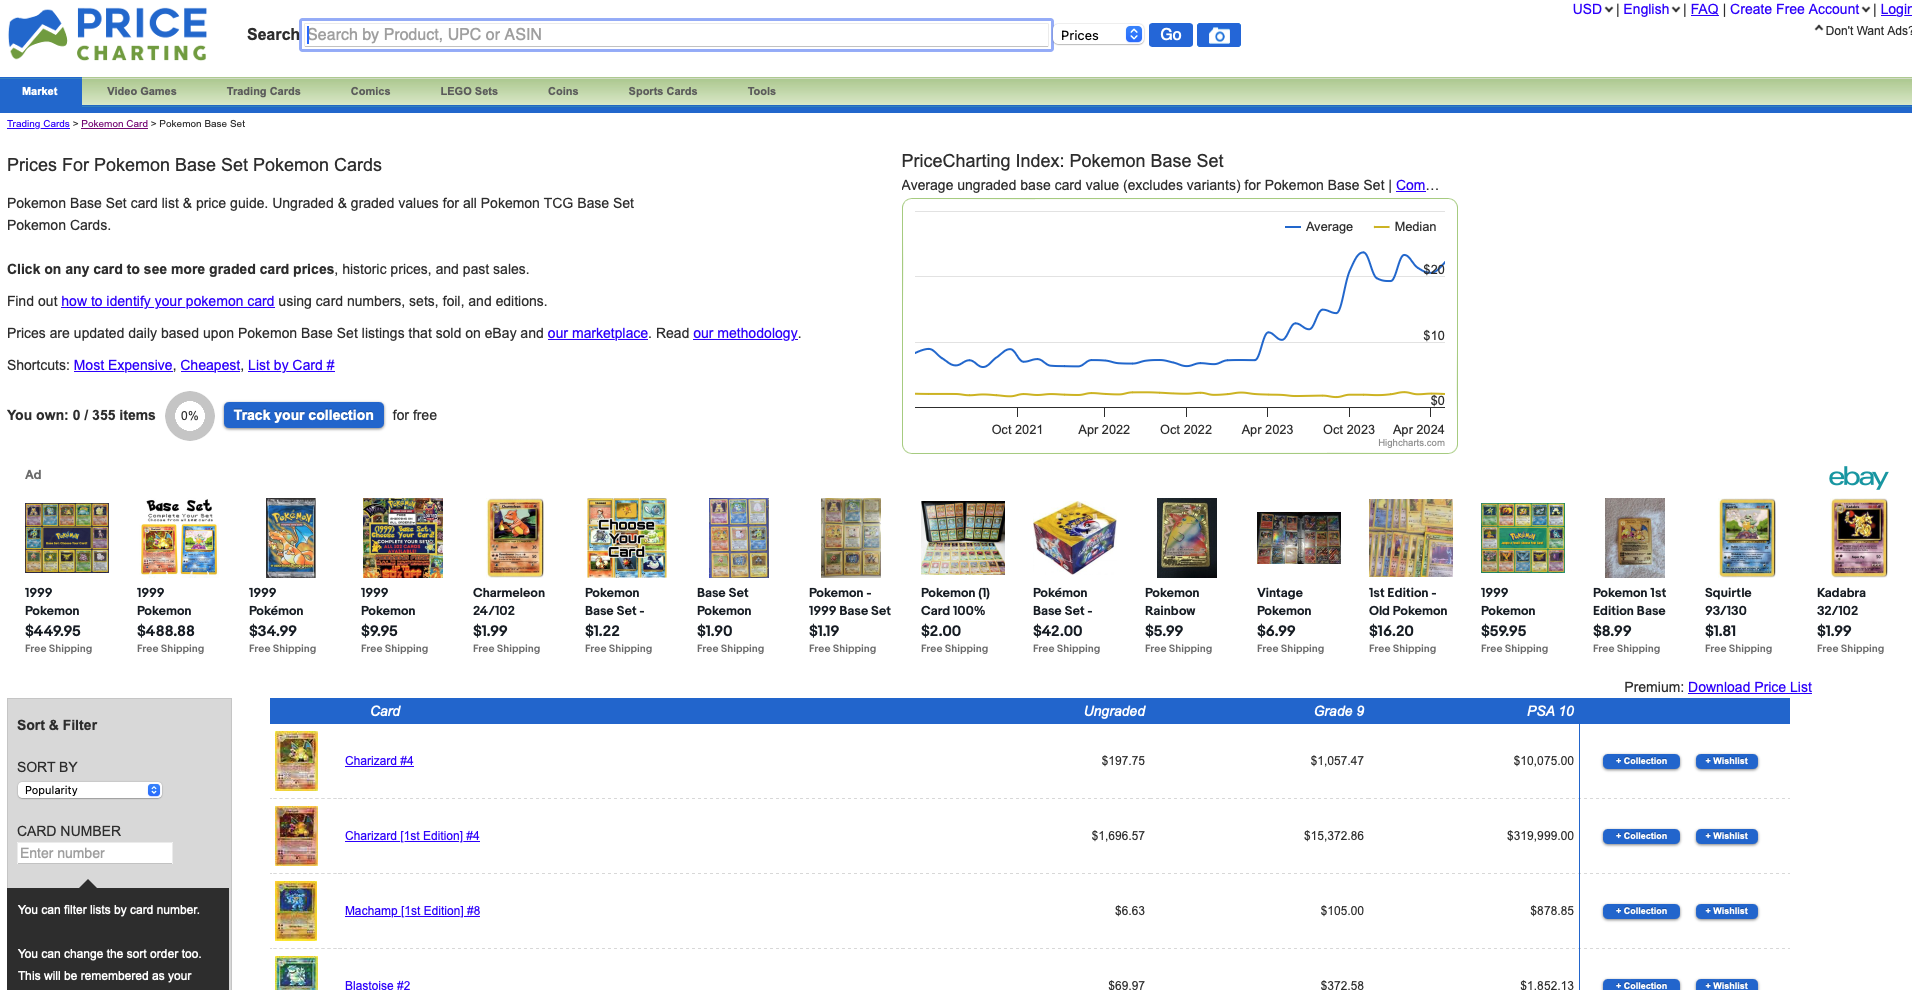
\includegraphics[width=0.9\textwidth]{figures/4-Estudio-viabilidad/4_PriceCharting.png}
    \caption{Página de cartas de Pokémon de PriceCharting}
    \label{fig:pricecharting}
    \hypertarget{fig:pricecharting}{}
\end{figure}

PriceCharting también proporciona información detallada sobre cada transacción y su precio, como se muestra en la \coloredUnderline{\hyperlink{fig:pricecharting2}{Figura \ref*{fig:pricecharting2}:\nameref*{fig:pricecharting2}}}.

\begin{figure}[H]
    \centering
    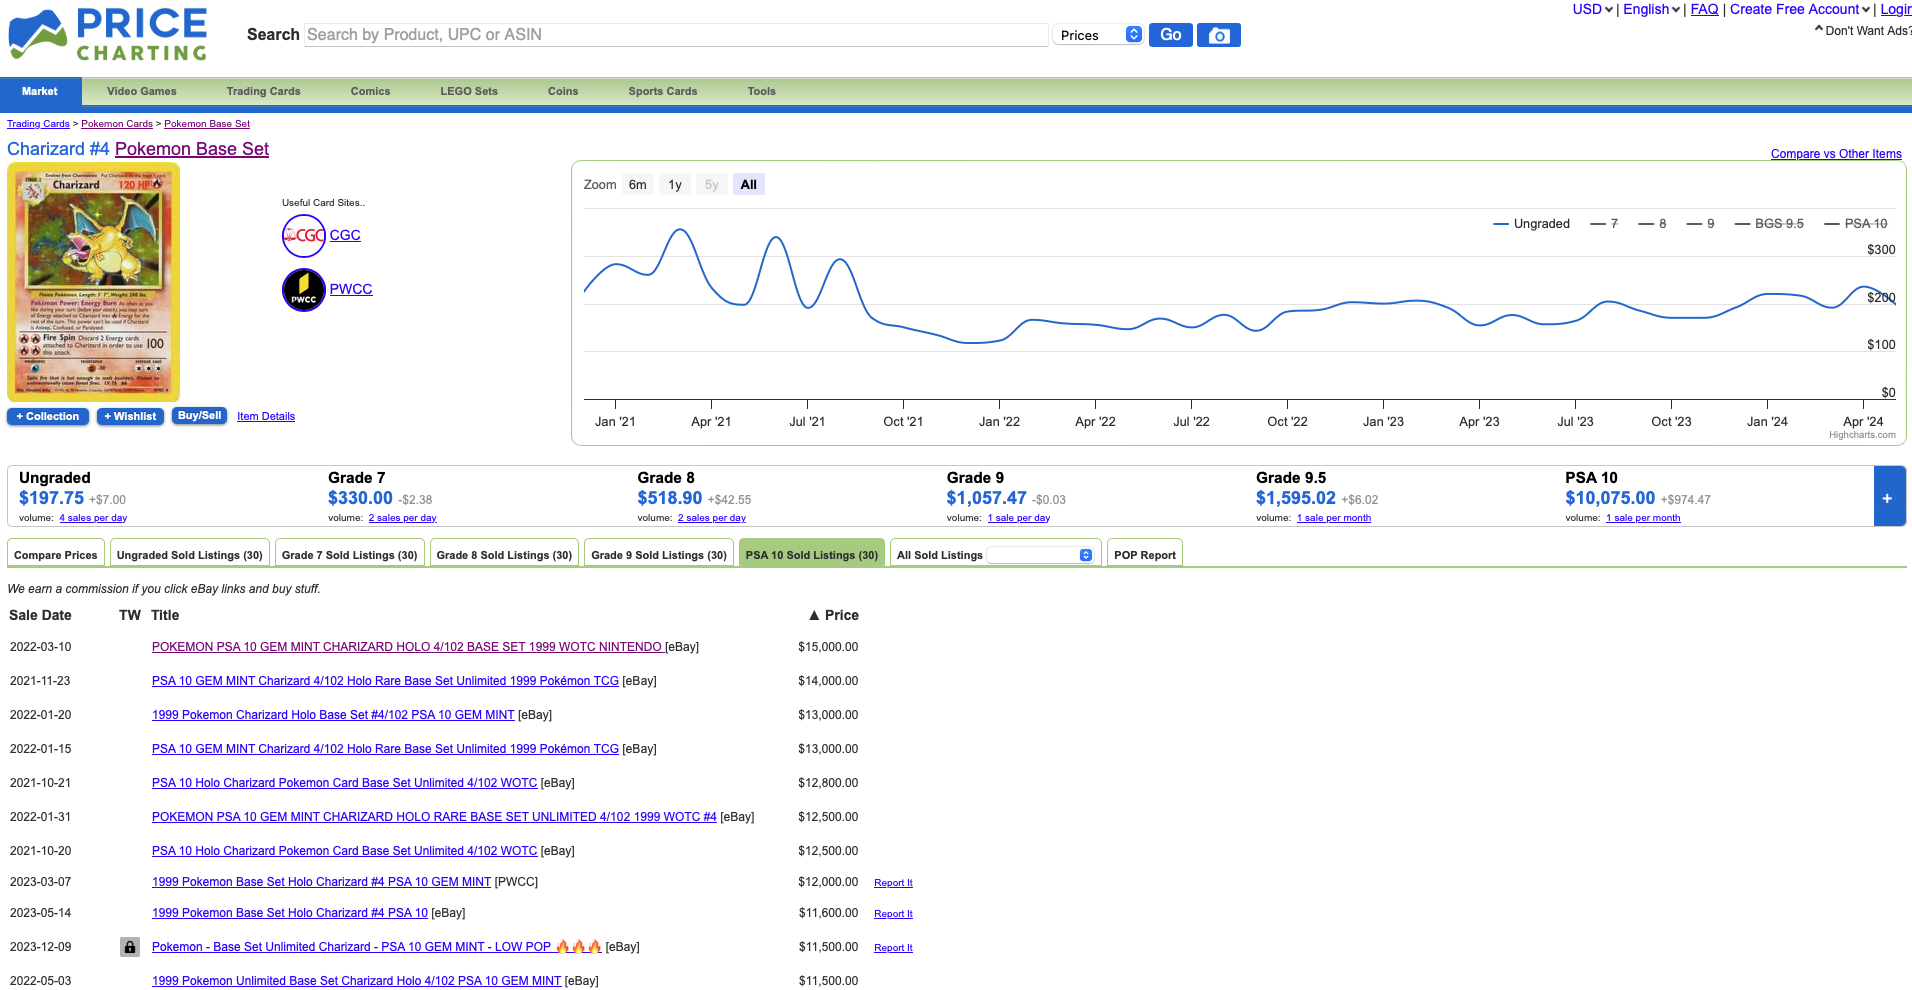
\includegraphics[width=0.9\textwidth]{figures/4-Estudio-viabilidad/4_PriceCharting2.png}
    \caption{Página de una carta de Pokémon de PriceCharting}
    \label{fig:pricecharting2}
    \hypertarget{fig:pricecharting2}{}
\end{figure}

El análisis de los datos recopilados en estas plataformas revela que el precio de las cartas de Pokémon varía en función de su rareza, estado de conservación y popularidad. 
Es evidente que el mercado de coleccionistas de Pokémon es un sector en constante crecimiento y expansión, generando una gran cantidad de ingresos, 
lo que lo convierte en un mercado altamente atractivo para su explotación.
